\chapter{Object Performance}\label{c:OP}

Prior to conducting a full study of TLA on the \VBFHBB channel, the features of jet objects reconstructed offline and within the HLT were compared to identify any performance differences in the base components of an event reconstruction. The jet objects were compared on a one to one basis, by matching an online jet to an offline jet by requiring the $\Delta R$ value between the two jets to be below a threshold value of \DELTARTHRESHOLD\footnote{Determined from a plot of $\Delta R$ values between all pairs of jets}. \todo{Does this need a plot, or is this sufficient?}

\section{Leading \textit{b}-jets}
\label{OP:leadingb}

	The leading \pt offline $b$-jet selected using the \textit{Tight} working point was matched to a corresponding $b$-jet using $\Delta R$ matching. The following figures show the ratio of the difference in value between the offline and online jet calculated using the following formula for jet feature $X$:

	\begin{equation}
	\Delta X_{ratio} = \frac{X_{Offline} - X_{Online}}{X_{Offline}}
	\end{equation}
	
	where $X_{Offline}$ is the value of the feature on the offline jet, and $X_{Online}$ is from the HLT jet.
	
	\newpage
	\subsection{Monte-Carlo}
	
		\subsubsection{Plots of \textit{b}-jet features}
		
		\begin{figure}[h]
			\centering
			\begin{minipage}[h]{0.33\linewidth}
				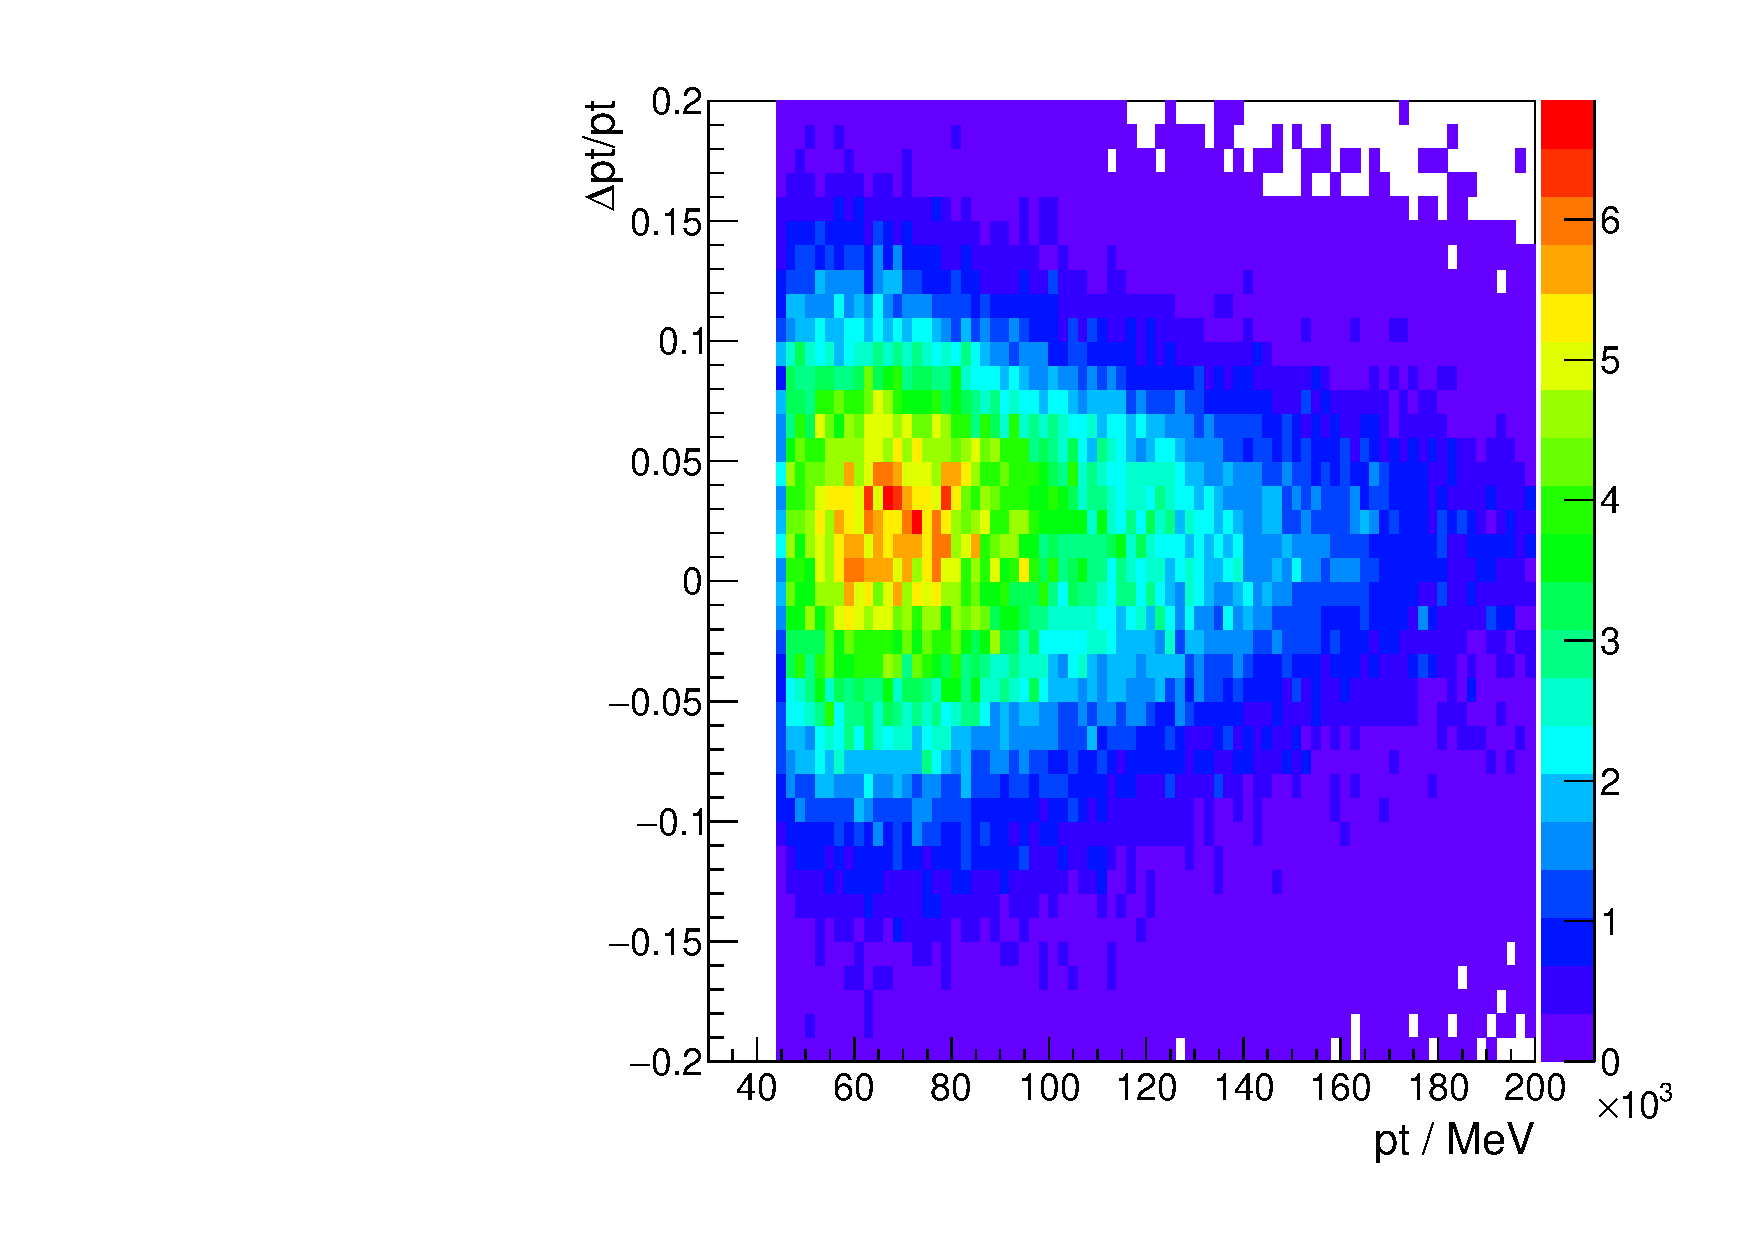
\includegraphics[width=1\linewidth]{ptRatio_Leading_BJet}
	
			\end{minipage}
			\quad
			\begin{minipage}[h]{0.33\linewidth}
				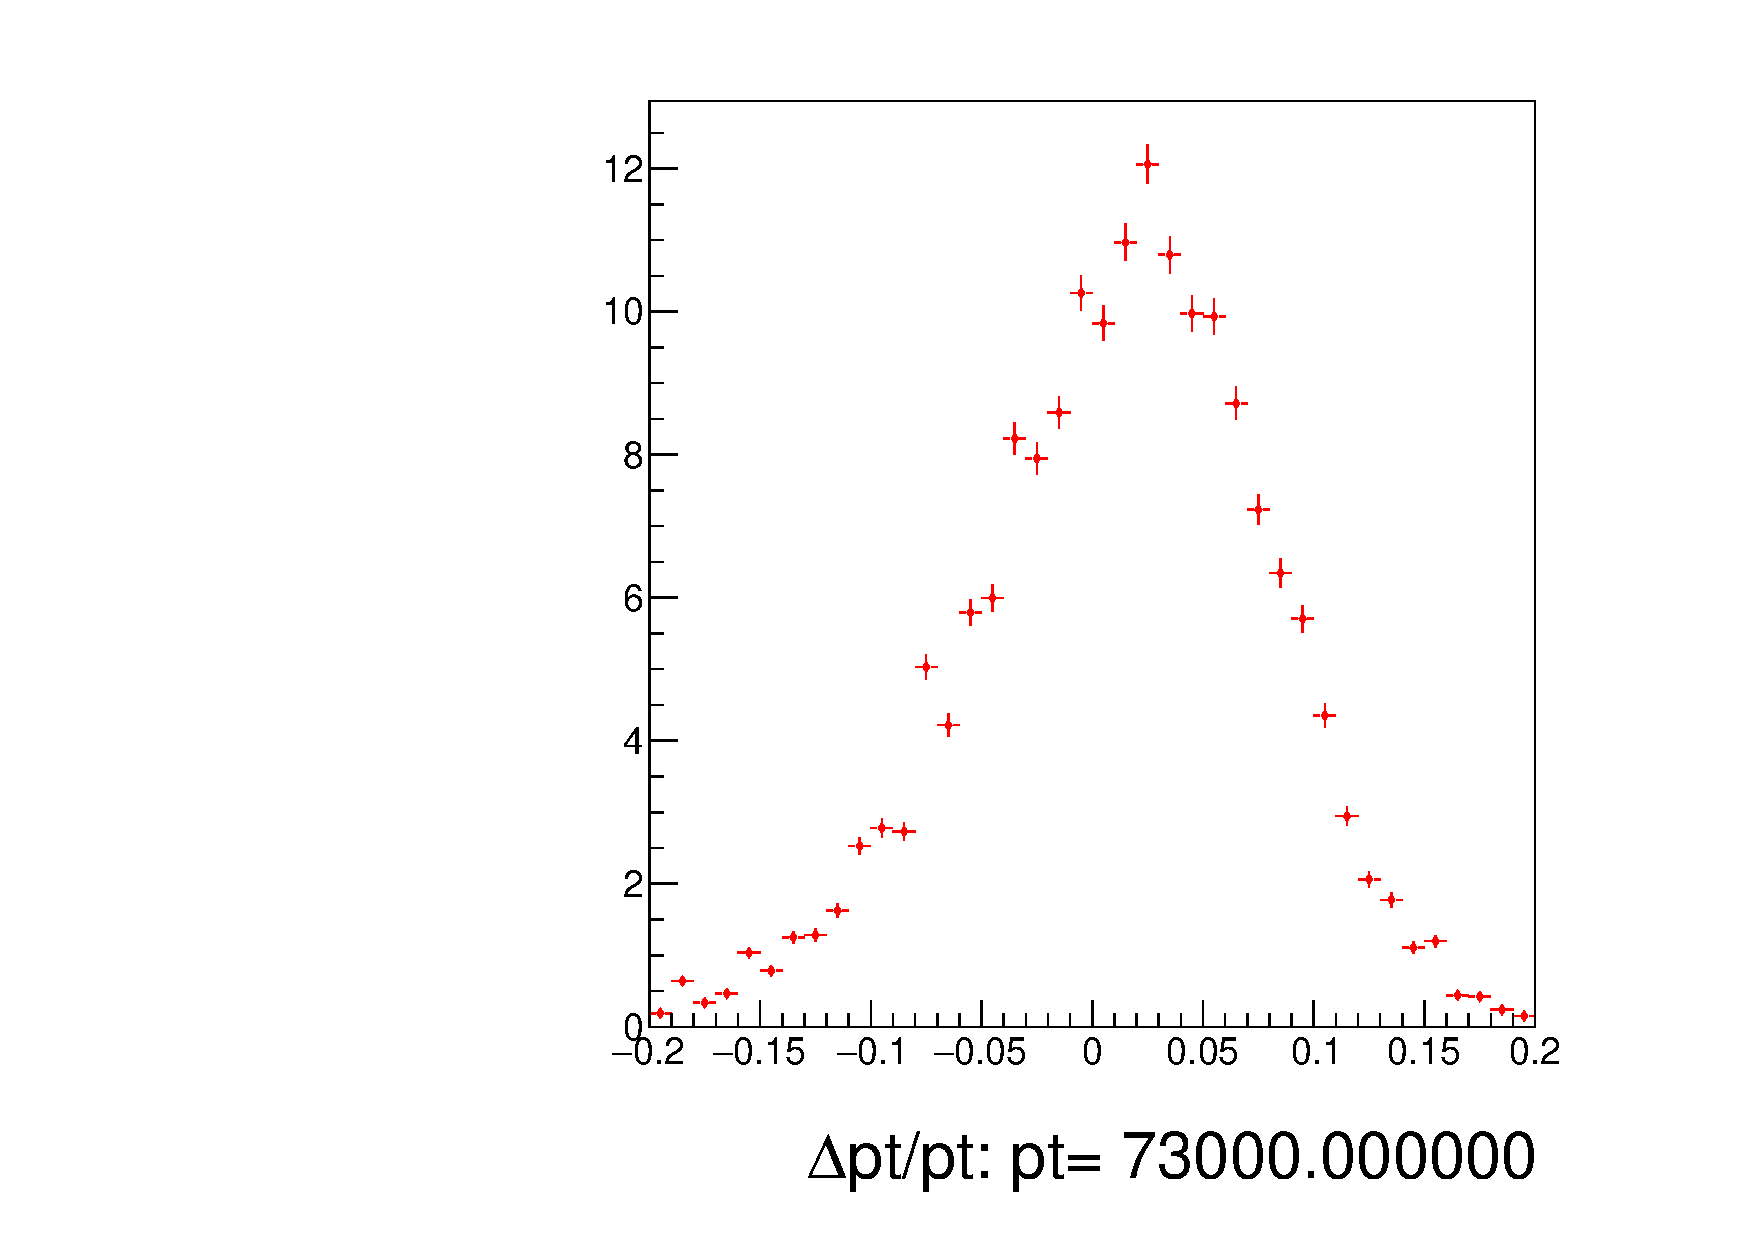
\includegraphics[width=1\linewidth]{ptRatio_Leading_BJet_Slice}
			\end{minipage}
			\caption{$\Delta $\pt$_{ratio}$ for the leading \pt $b$-jet from MC events against \pt of the offline $b$-jet. A slice across the $y$-axis has been taken at \pt$=79$GeV. }
			\label{fig:MC:leadingbpt}
		\end{figure}
		
		\begin{figure}[h]
			\centering
			
			\begin{minipage}[h]{0.33\linewidth}
				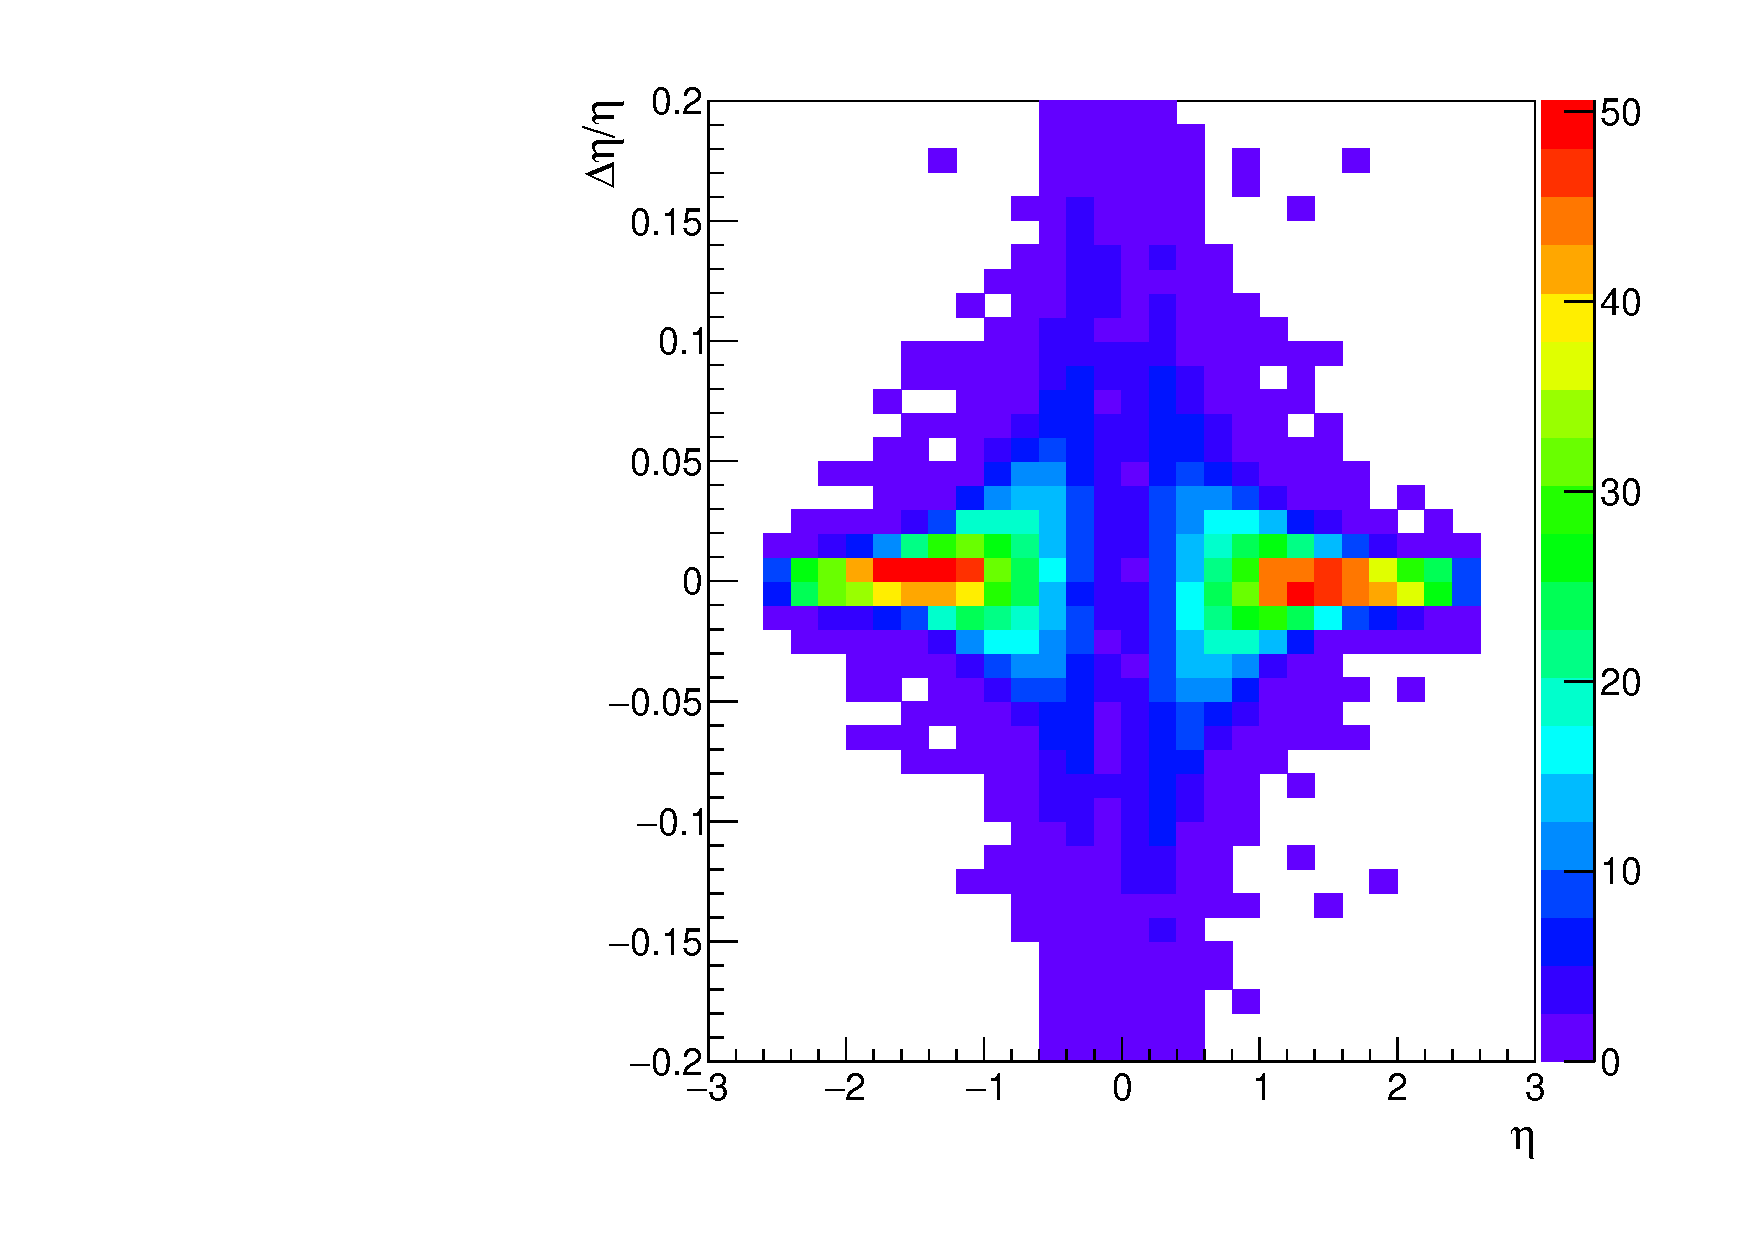
\includegraphics[width=1\linewidth]{etaRatio_Leading_BJet}
			\end{minipage}
			\quad
			\begin{minipage}[h]{0.33\linewidth}
				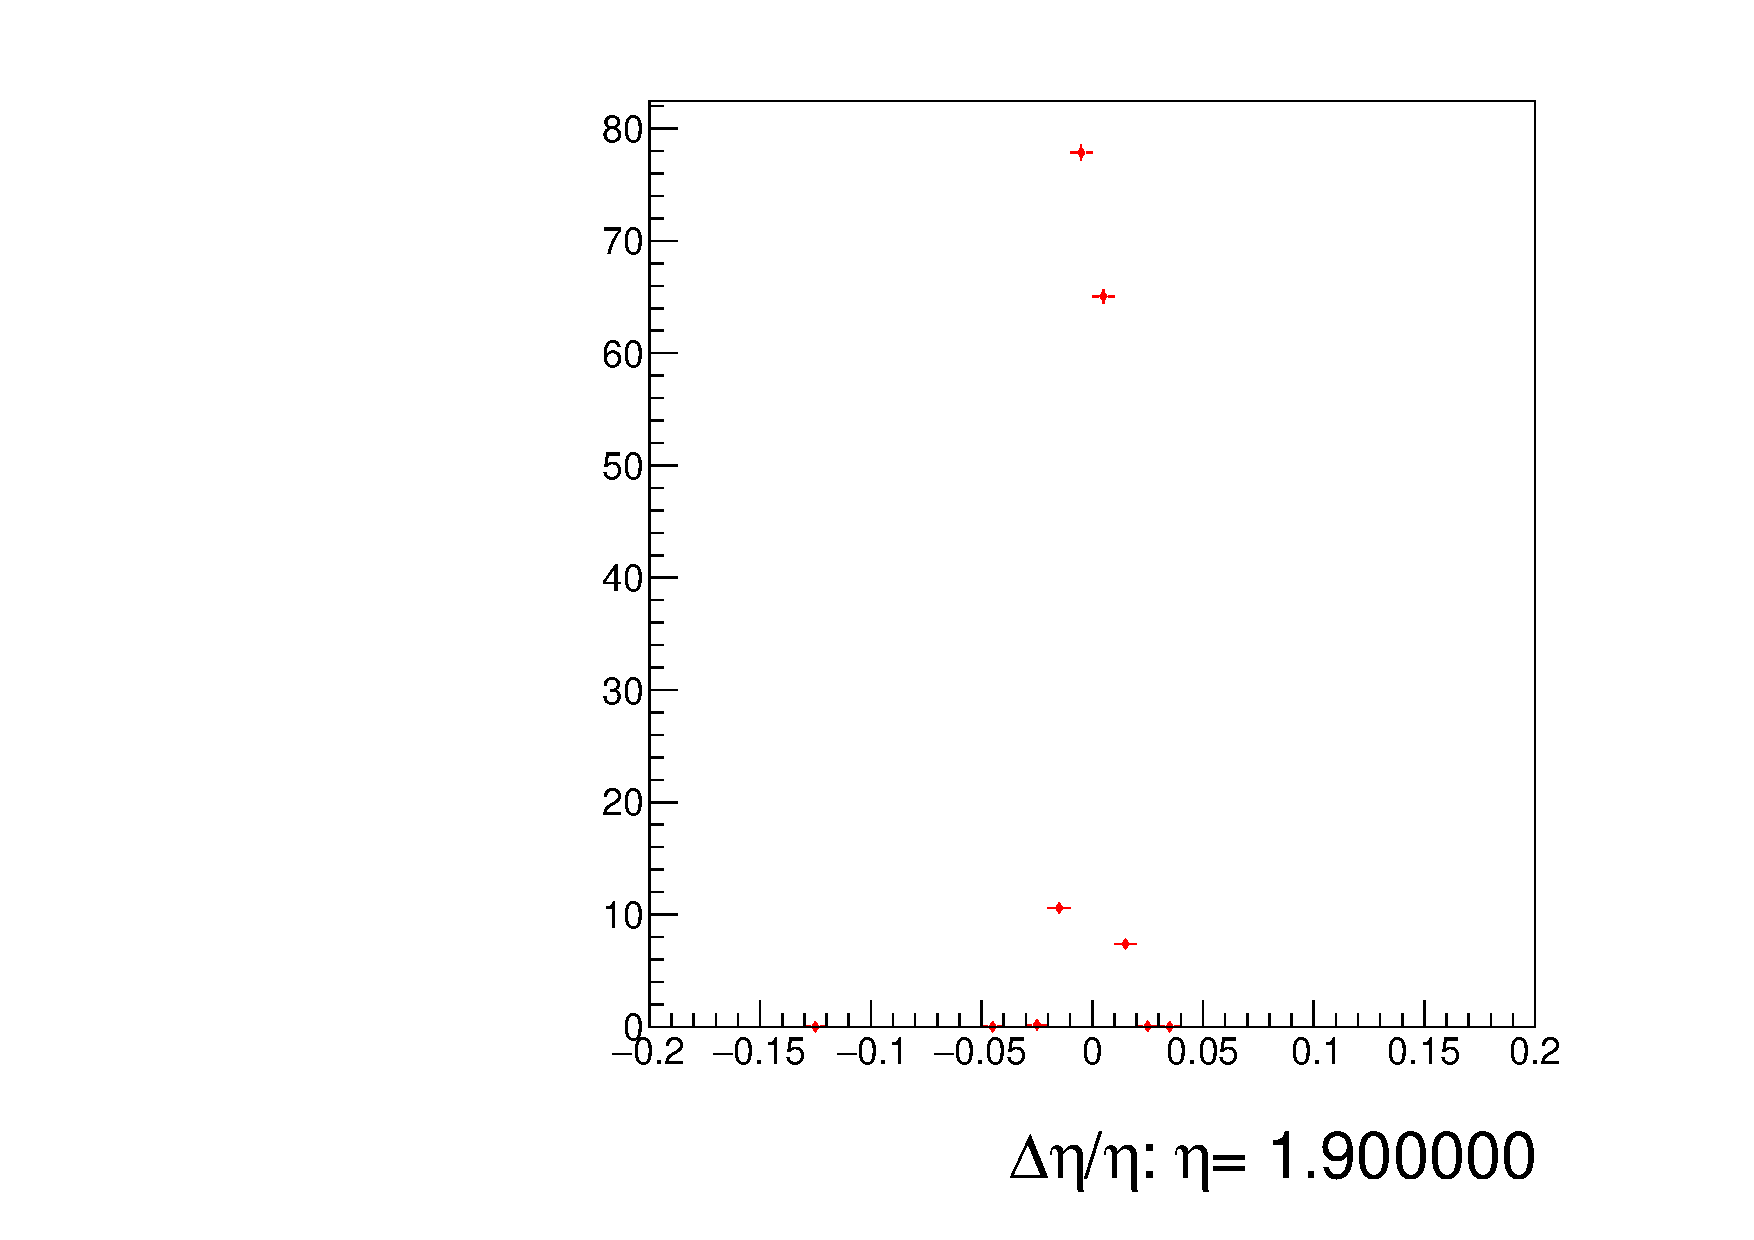
\includegraphics[width=1\linewidth]{etaRatio_Leading_BJet_Slice}
			\end{minipage}
			\caption{$\Delta \eta_{ratio}$ for the leading \pt $b$-jet from MC events against $\eta$ of the offline $b$-jet. A slice across the $y$-axis has been taken at $\eta=-1.9$. }
			\label{fig:MC:leadingbeta}
		\end{figure}
		
			\begin{figure}[h]
				\centering
				
				\begin{minipage}[h]{0.33\linewidth}
					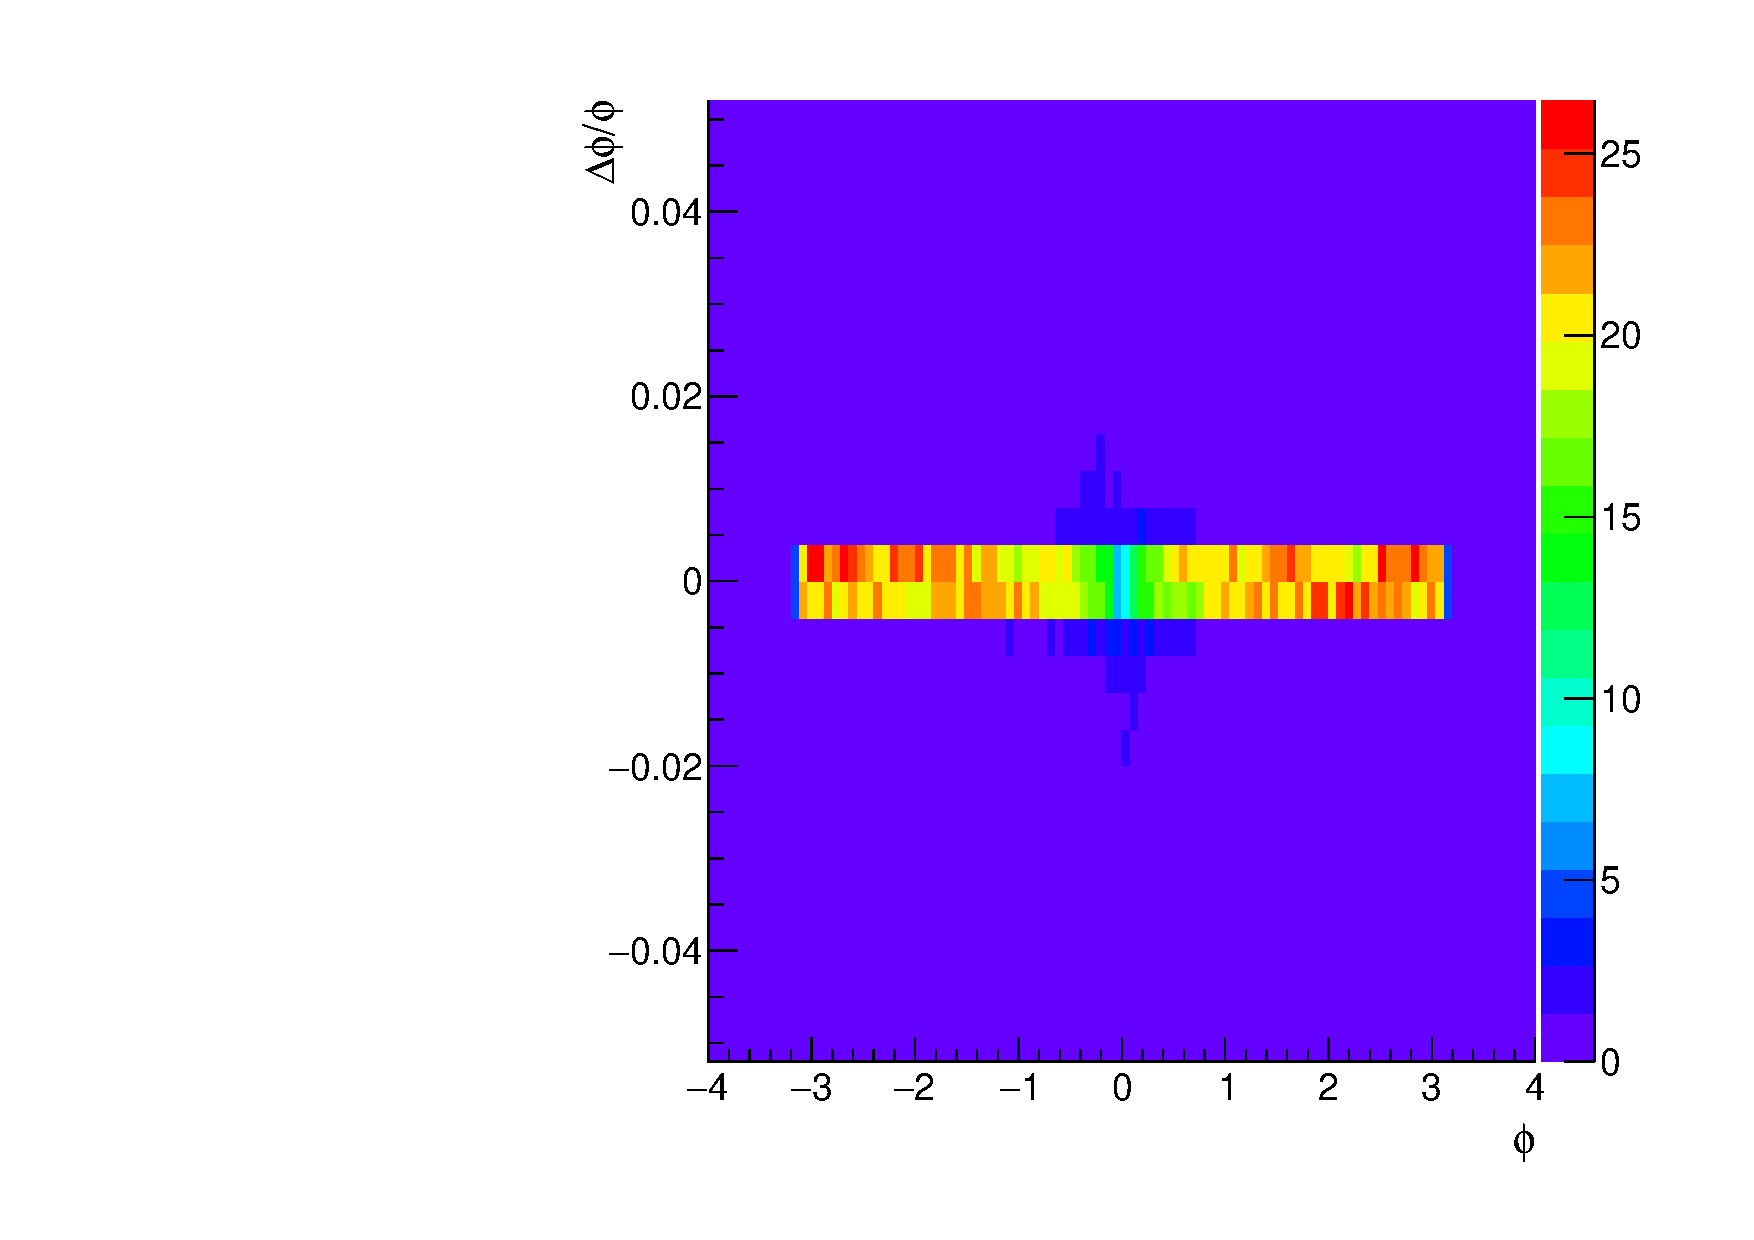
\includegraphics[width=1\linewidth]{phiRatio_Leading_BJet}
				\end{minipage}
				\quad
				\begin{minipage}[h]{0.33\linewidth}
					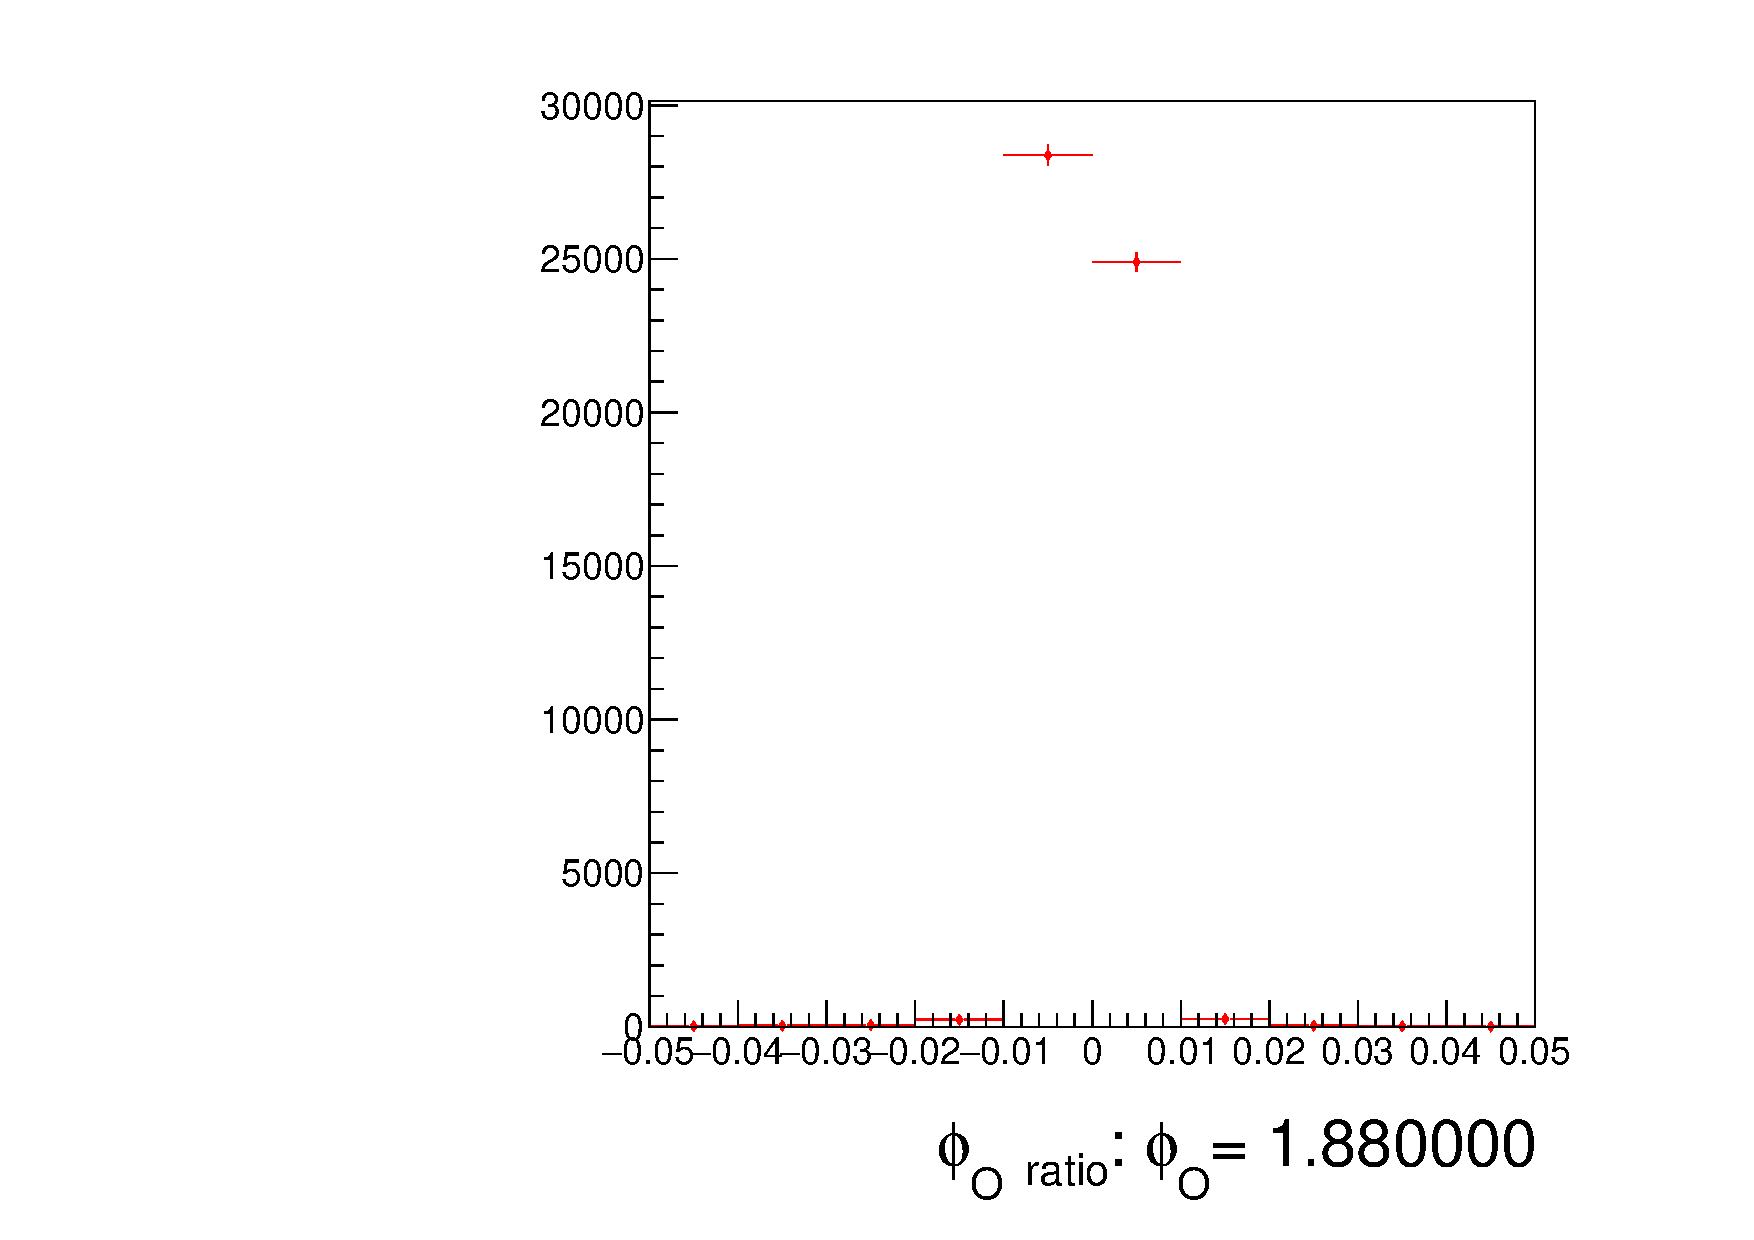
\includegraphics[width=1\linewidth]{phiRatio_Leading_BJet_Slice}
				\end{minipage}
			\caption{$\Delta \phi_{ratio}$ for the leading \pt $b$-jet from MC events against $\phi$ of the offline $b$-jet. A slice across the $y$-axis has been taken at $\phi=-1.64$. }
			\label{fig:MC:leadingbphi}
			\end{figure}
			
			\begin{figure}[h]
				\centering
				
				\begin{minipage}[h]{0.33\linewidth}
					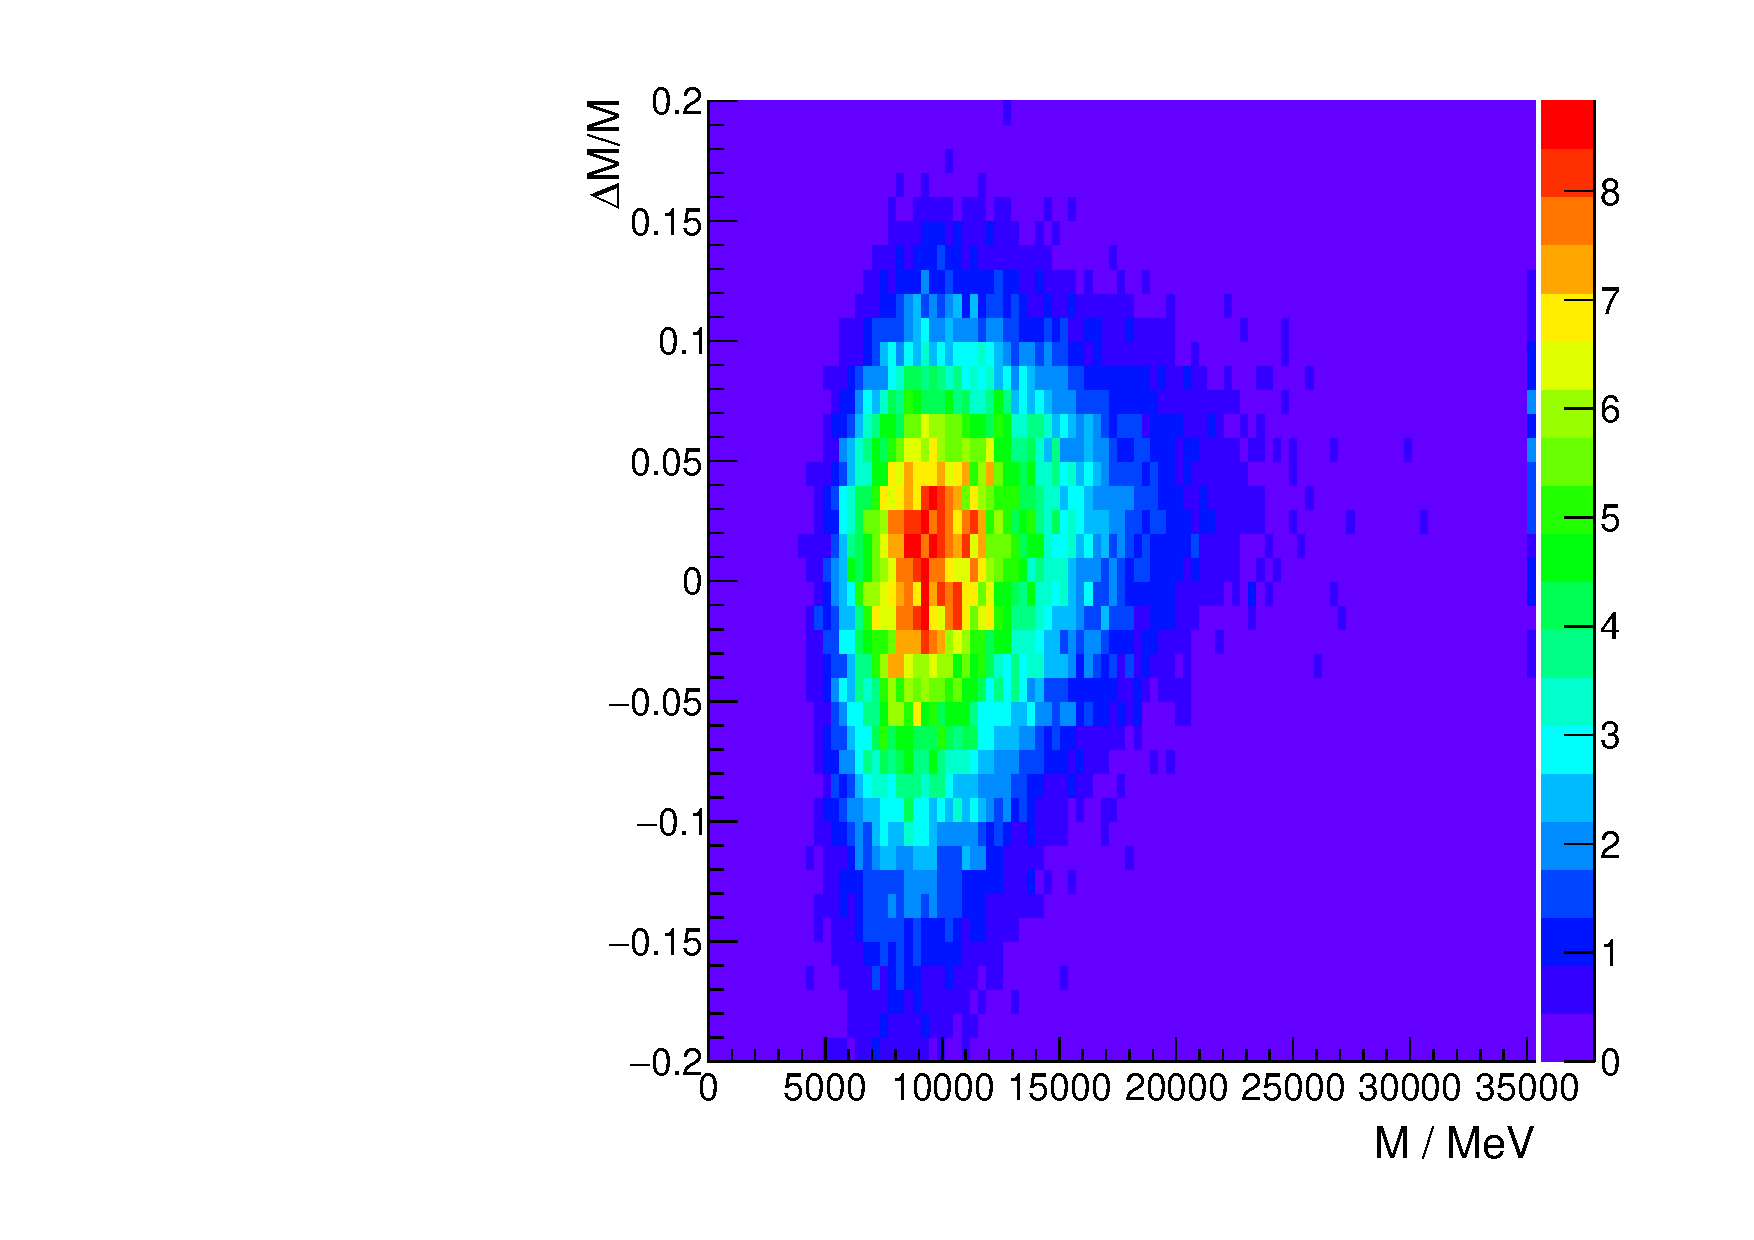
\includegraphics[width=1\linewidth]{mRatio_Leading_BJet}
				\end{minipage}
				\quad
				\begin{minipage}[h]{0.33\linewidth}
					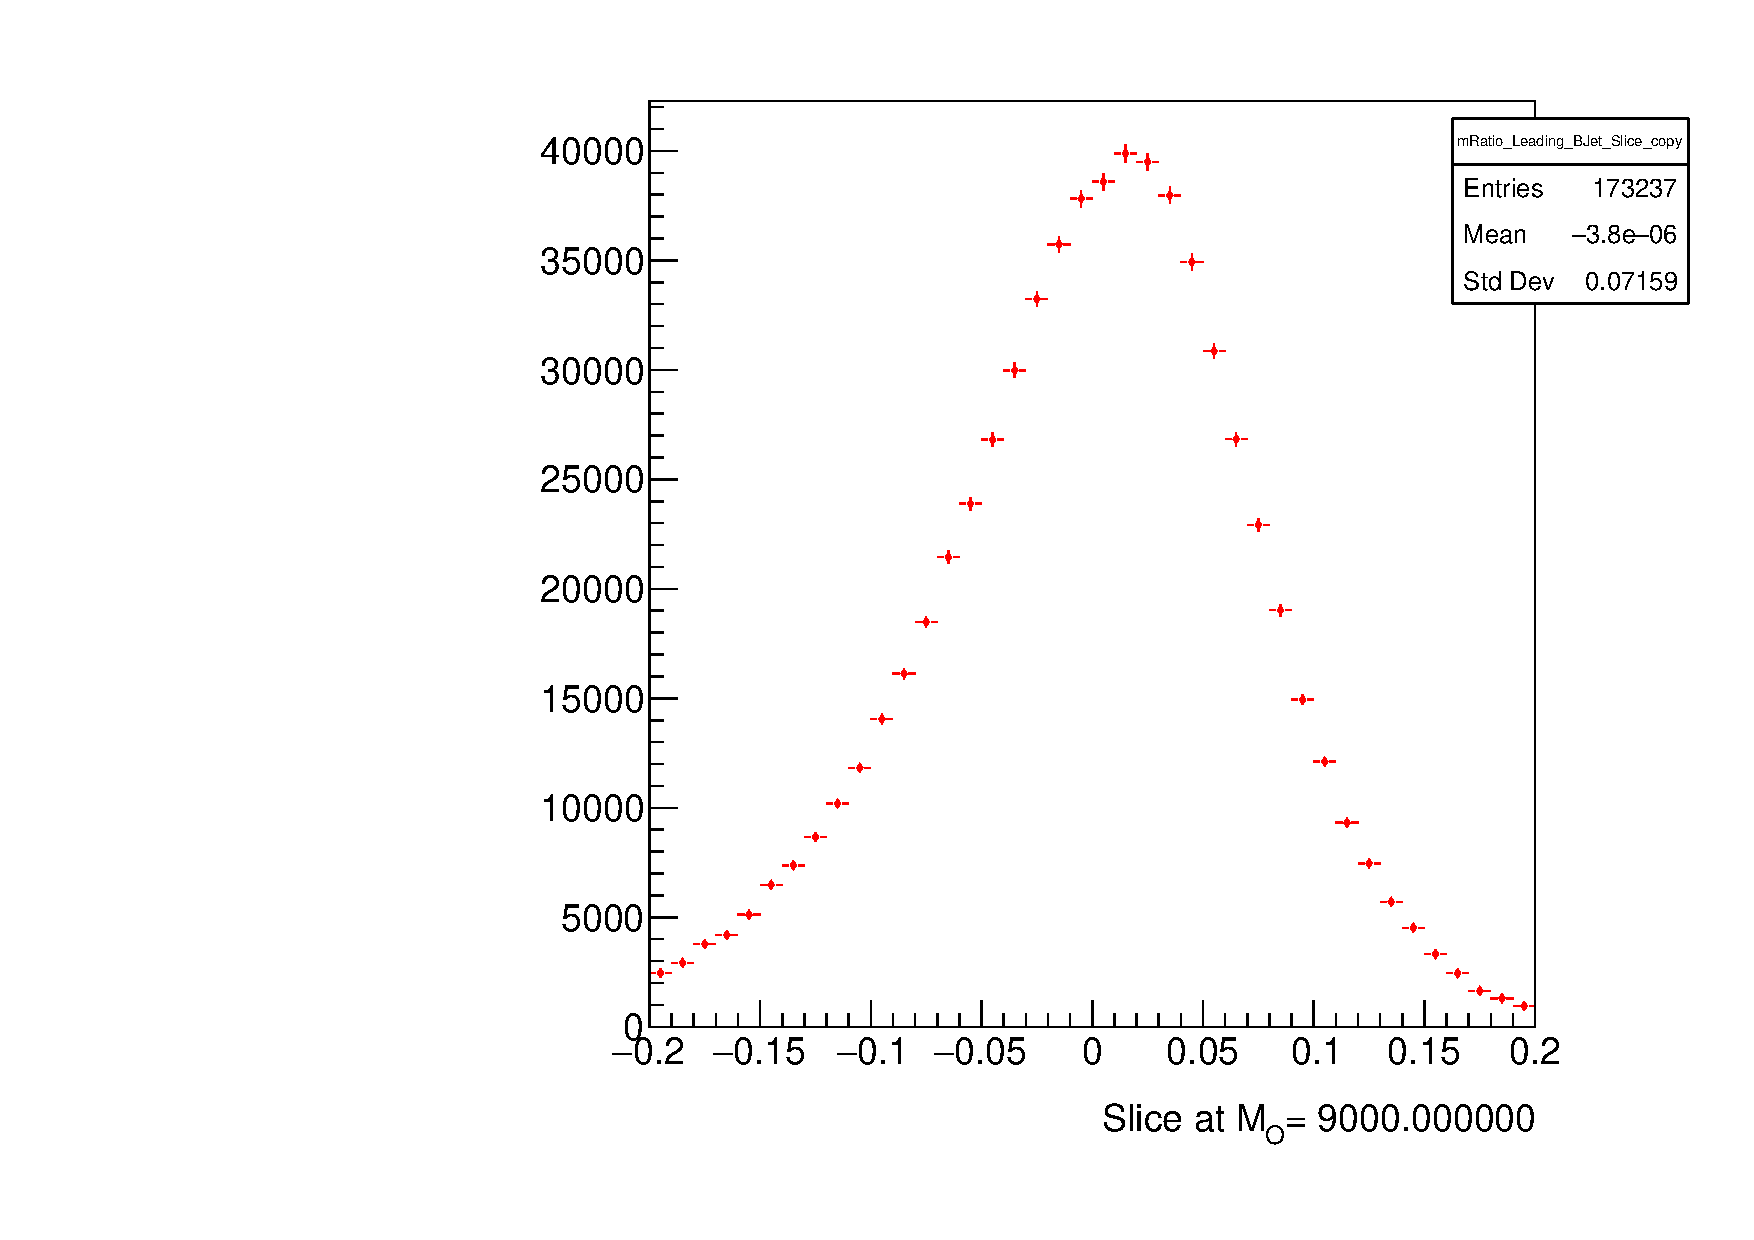
\includegraphics[width=1\linewidth]{mRatio_Leading_BJet_Slice}
				\end{minipage}
			\caption{$\Delta M_{ratio}$ for the leading \pt $b$-jet from MC events against $M$ of the offline $b$-jet. A slice across the $y$-axis has been taken at $M=7$GeV. }
			\label{fig:MC:leadingbm}
			\end{figure}
			
		\subsubsection{Conclusions from MC jet features}
	
	\newpage
	\subsection{Data}
	
	\begin{figure}[h]
		\centering
		
		\begin{minipage}[h]{0.33\linewidth}
			
\includegraphics[width=1\linewidth]{placeholder}
			\caption{}
			\label{fig:D:leadingbpt}
		\end{minipage}
		\quad
		\begin{minipage}[h]{0.33\linewidth}
			
\includegraphics[width=1\linewidth]{placeholder}
			\caption{}
			\label{fig:D:leadingbptslice}
		\end{minipage}
	\end{figure}
	
	\begin{figure}[h]
		\centering
		
		\begin{minipage}[h]{0.33\linewidth}
			
\includegraphics[width=1\linewidth]{placeholder}
			\caption{}
			\label{fig:D:leadingbeta}
		\end{minipage}
		\quad
		\begin{minipage}[h]{0.33\linewidth}
			
\includegraphics[width=1\linewidth]{placeholder}
			\caption{}
			\label{fig:D:leadingbetaslice}
		\end{minipage}
	\end{figure}
	
	\begin{figure}[h]
		\centering
		
		\begin{minipage}[h]{0.33\linewidth}
			
\includegraphics[width=1\linewidth]{placeholder}
			\caption{}
			\label{fig:D:leadingbphi}
		\end{minipage}
		\quad
		\begin{minipage}[h]{0.33\linewidth}
			
\includegraphics[width=1\linewidth]{placeholder}
			\caption{}
			\label{fig:D:leadingbphislice}
		\end{minipage}
	\end{figure}
	
	\begin{figure}[h]
		\centering
		
		\begin{minipage}[h]{0.33\linewidth}
			
\includegraphics[width=1\linewidth]{placeholder}
			\caption{}
			\label{fig:D:leadingbm}
		\end{minipage}
		\quad
		\begin{minipage}[h]{0.33\linewidth}
			
\includegraphics[width=1\linewidth]{placeholder}
			\caption{}
			\label{fig:D:leadingbmslice}
		\end{minipage}
	\end{figure}

\newpage
\section{Leading Non \textit{b}-jets}

	The non $b$-jet category is defined as the jets exclusive to those tagged in Section \ref{OP:leadingb}. Again, the leading \pt offline jet from this list is matched with an online jet for the comparison.

\newpage
	\subsection{Monte-Carlo}
	
		\begin{figure}[h]
			\centering
			\begin{minipage}[h]{0.33\linewidth}
				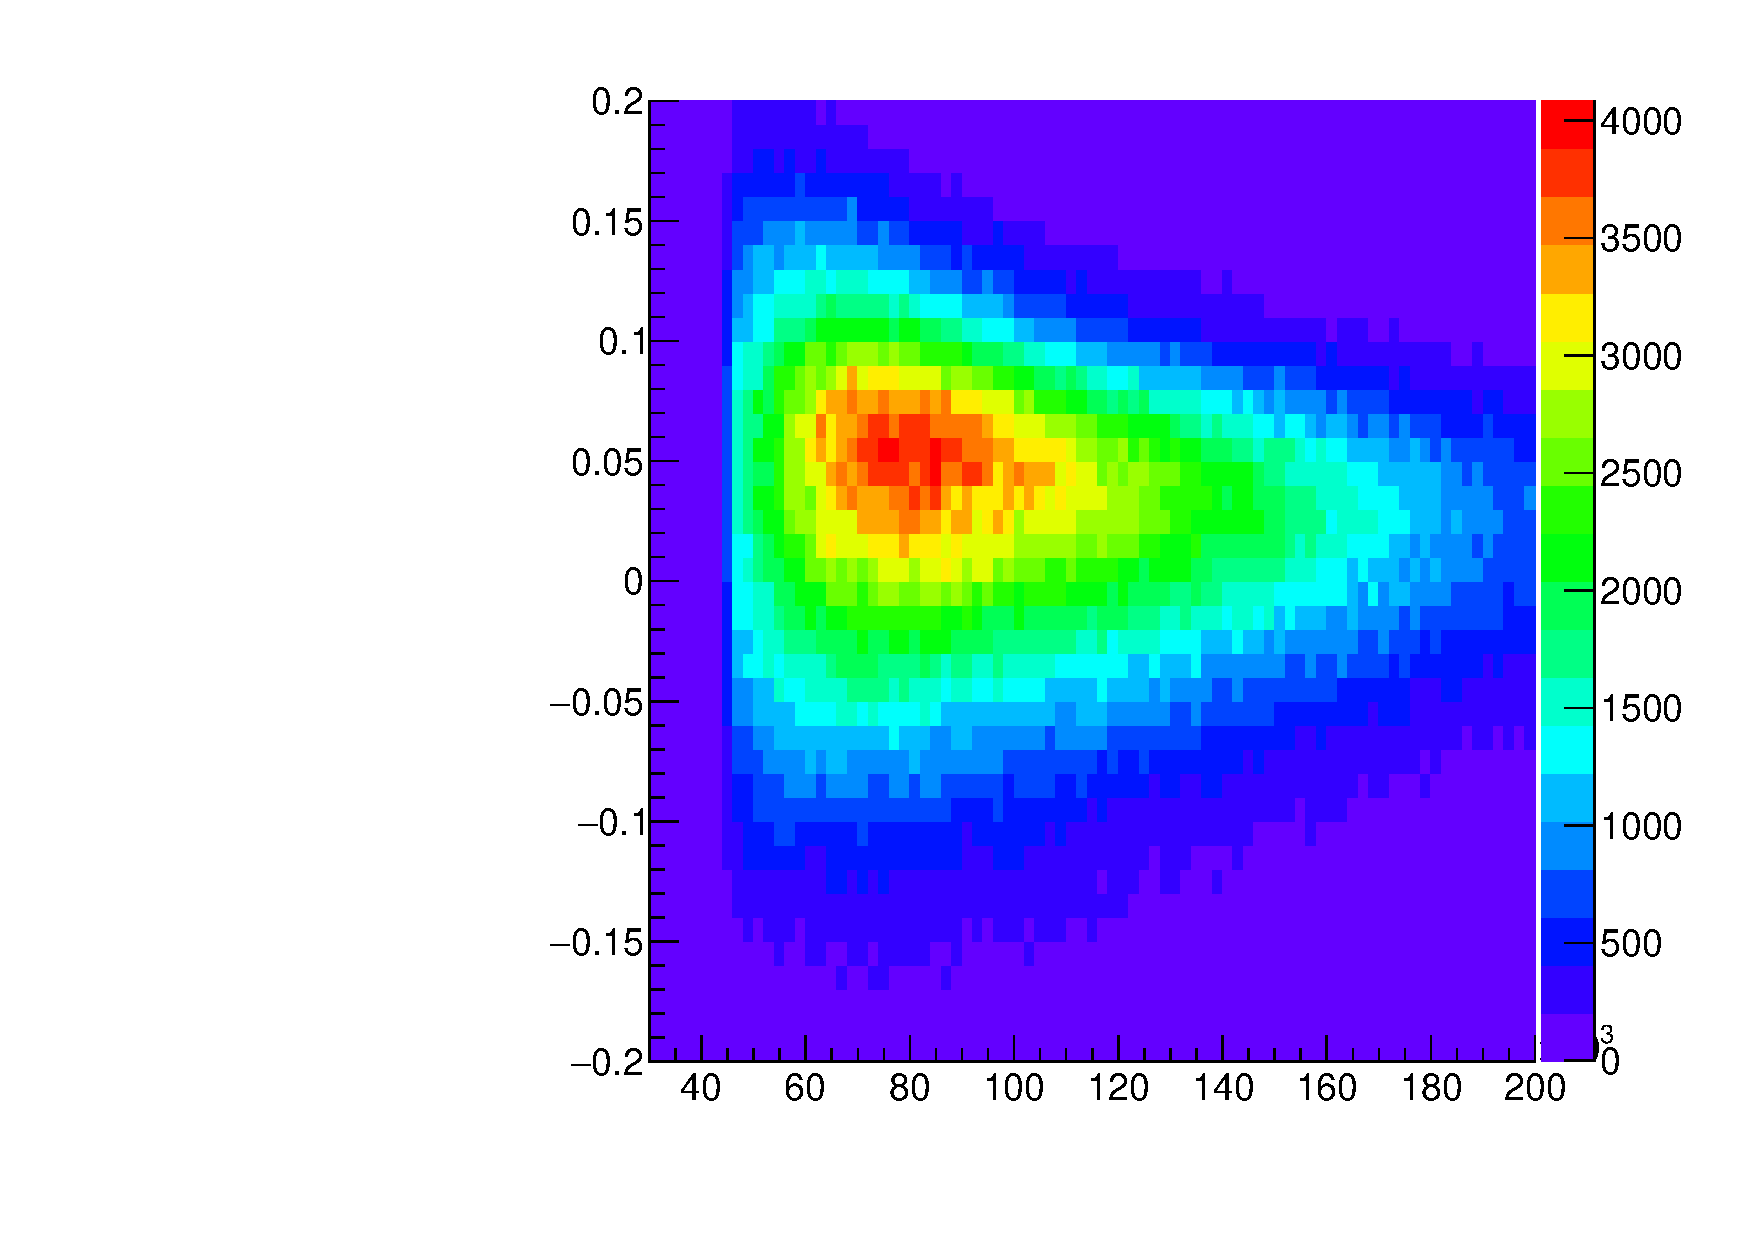
\includegraphics[width=1\linewidth]{ptRatio_Leading_Non_BJet}
				
			\end{minipage}
			\quad
			\begin{minipage}[h]{0.33\linewidth}
				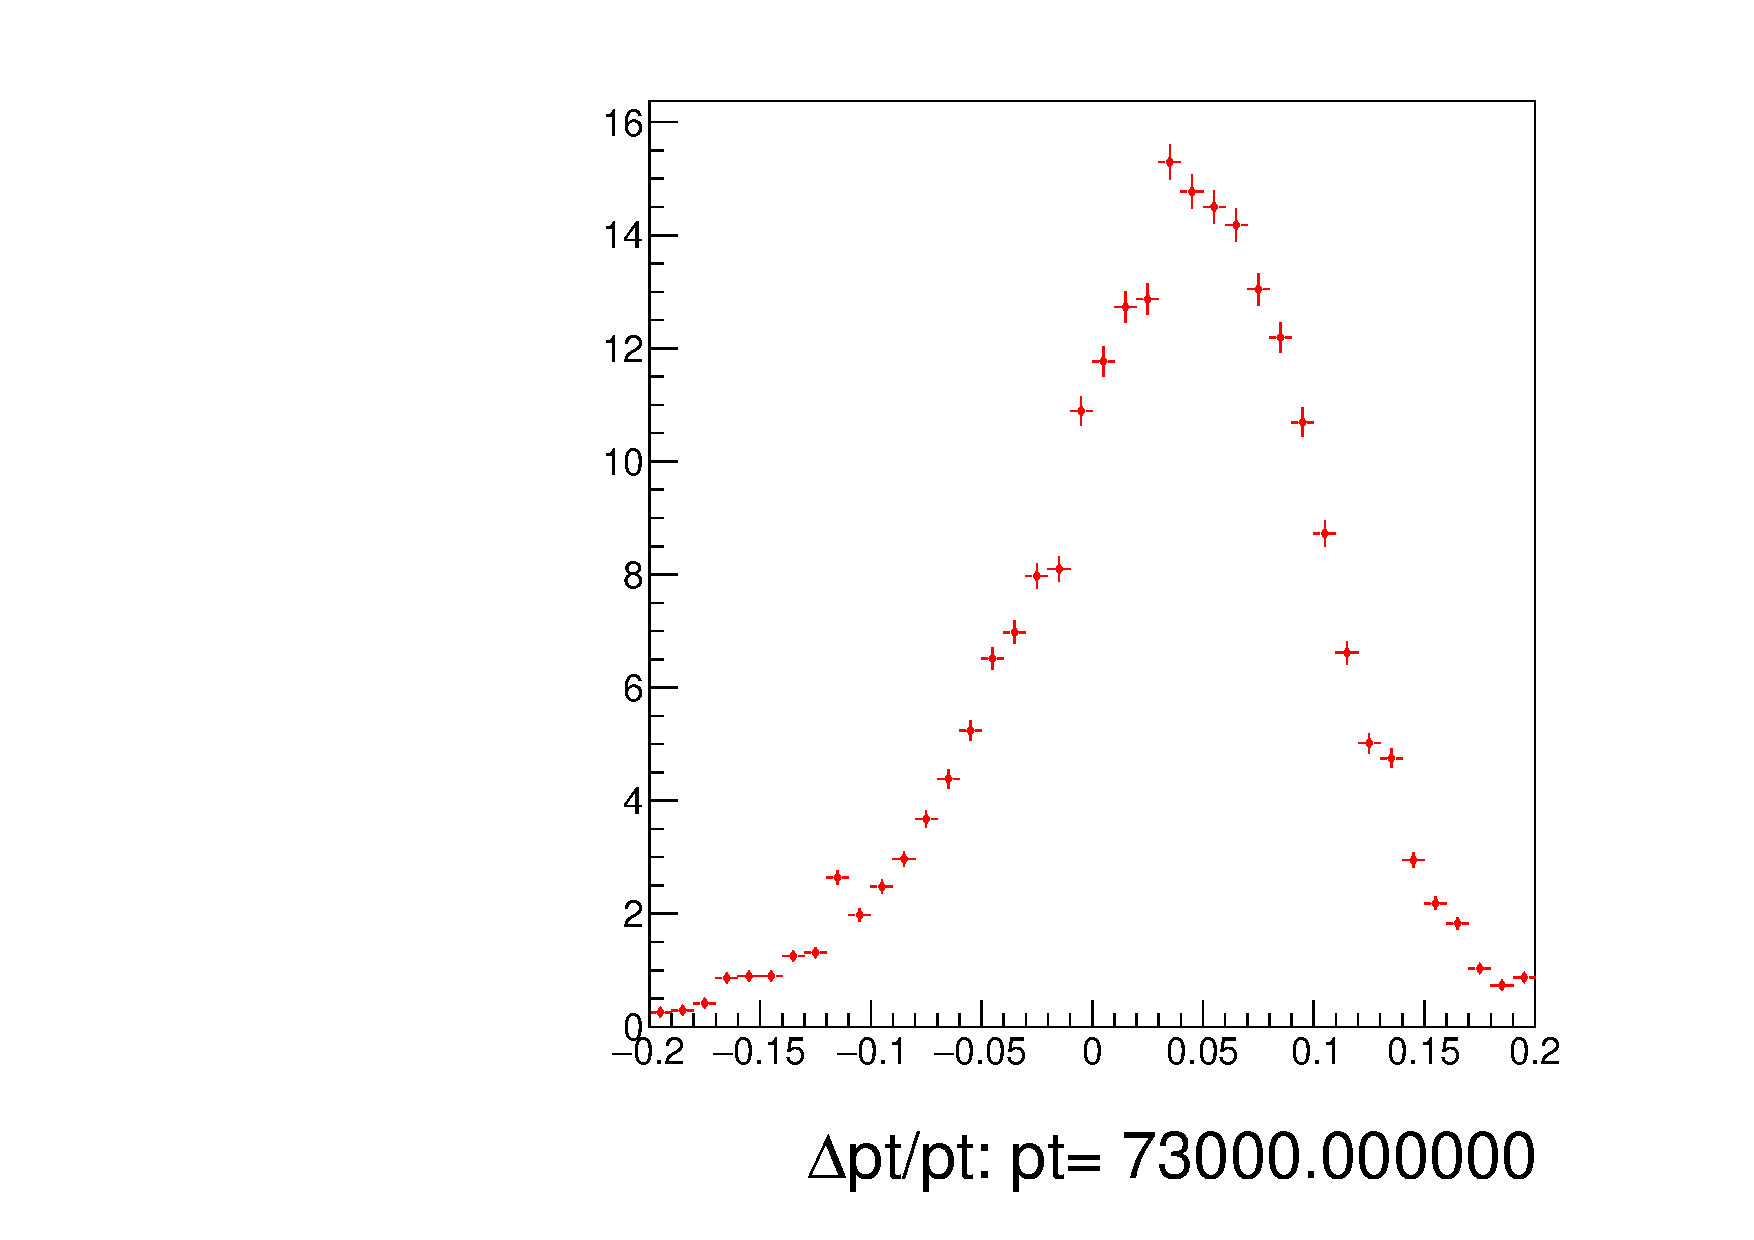
\includegraphics[width=1\linewidth]{ptRatio_Leading_Non_BJet_Slice}
			\end{minipage}
			\caption{$\Delta $\pt$_{ratio}$ for the leading \pt non $b$-jet from MC events against \pt of the offline $b$-jet. A slice across the $y$-axis has been taken at \pt$=79$GeV. }
			\label{fig:MC:nonleadingbpt}
		\end{figure}
		
		\begin{figure}[h]
			\centering
			
			\begin{minipage}[h]{0.33\linewidth}
				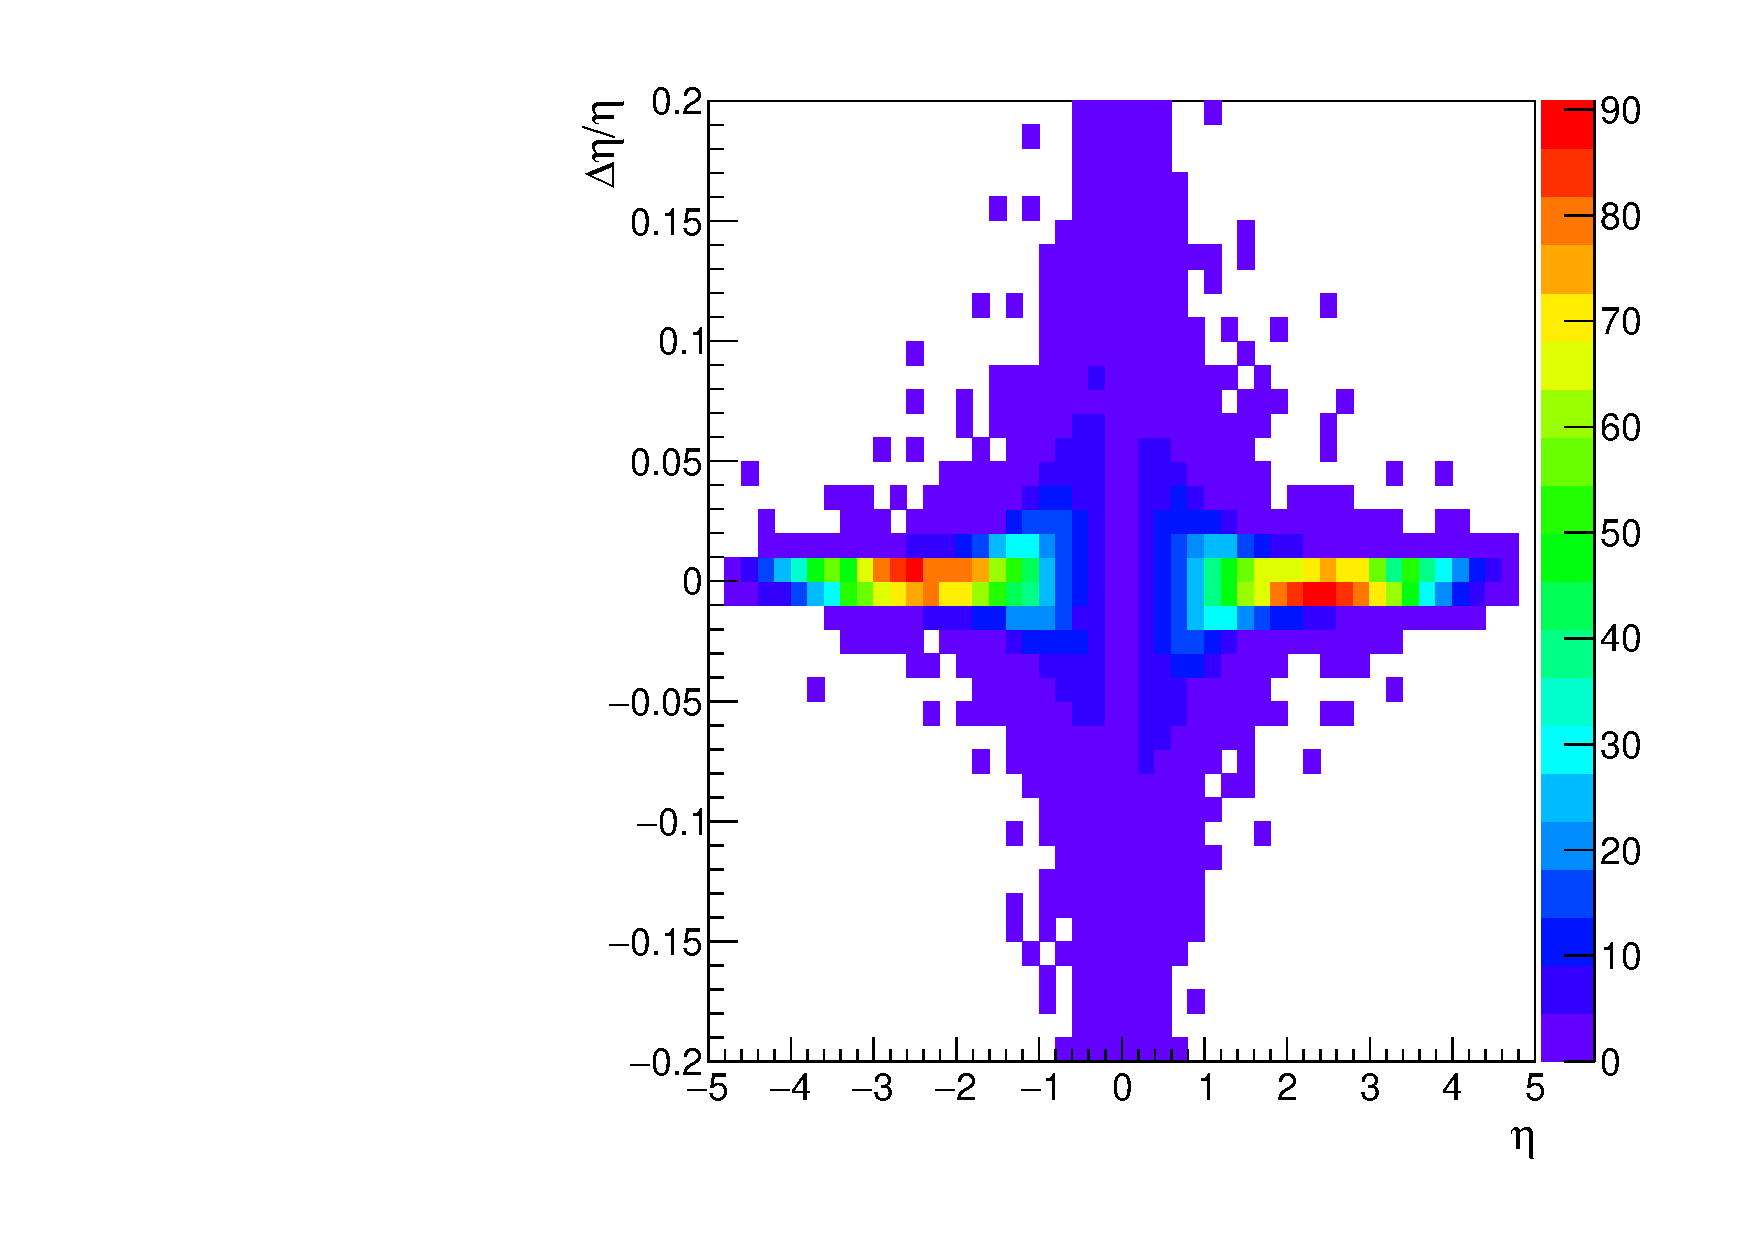
\includegraphics[width=1\linewidth]{etaRatio_Leading_Non_BJet}
			\end{minipage}
			\quad
			\begin{minipage}[h]{0.33\linewidth}
				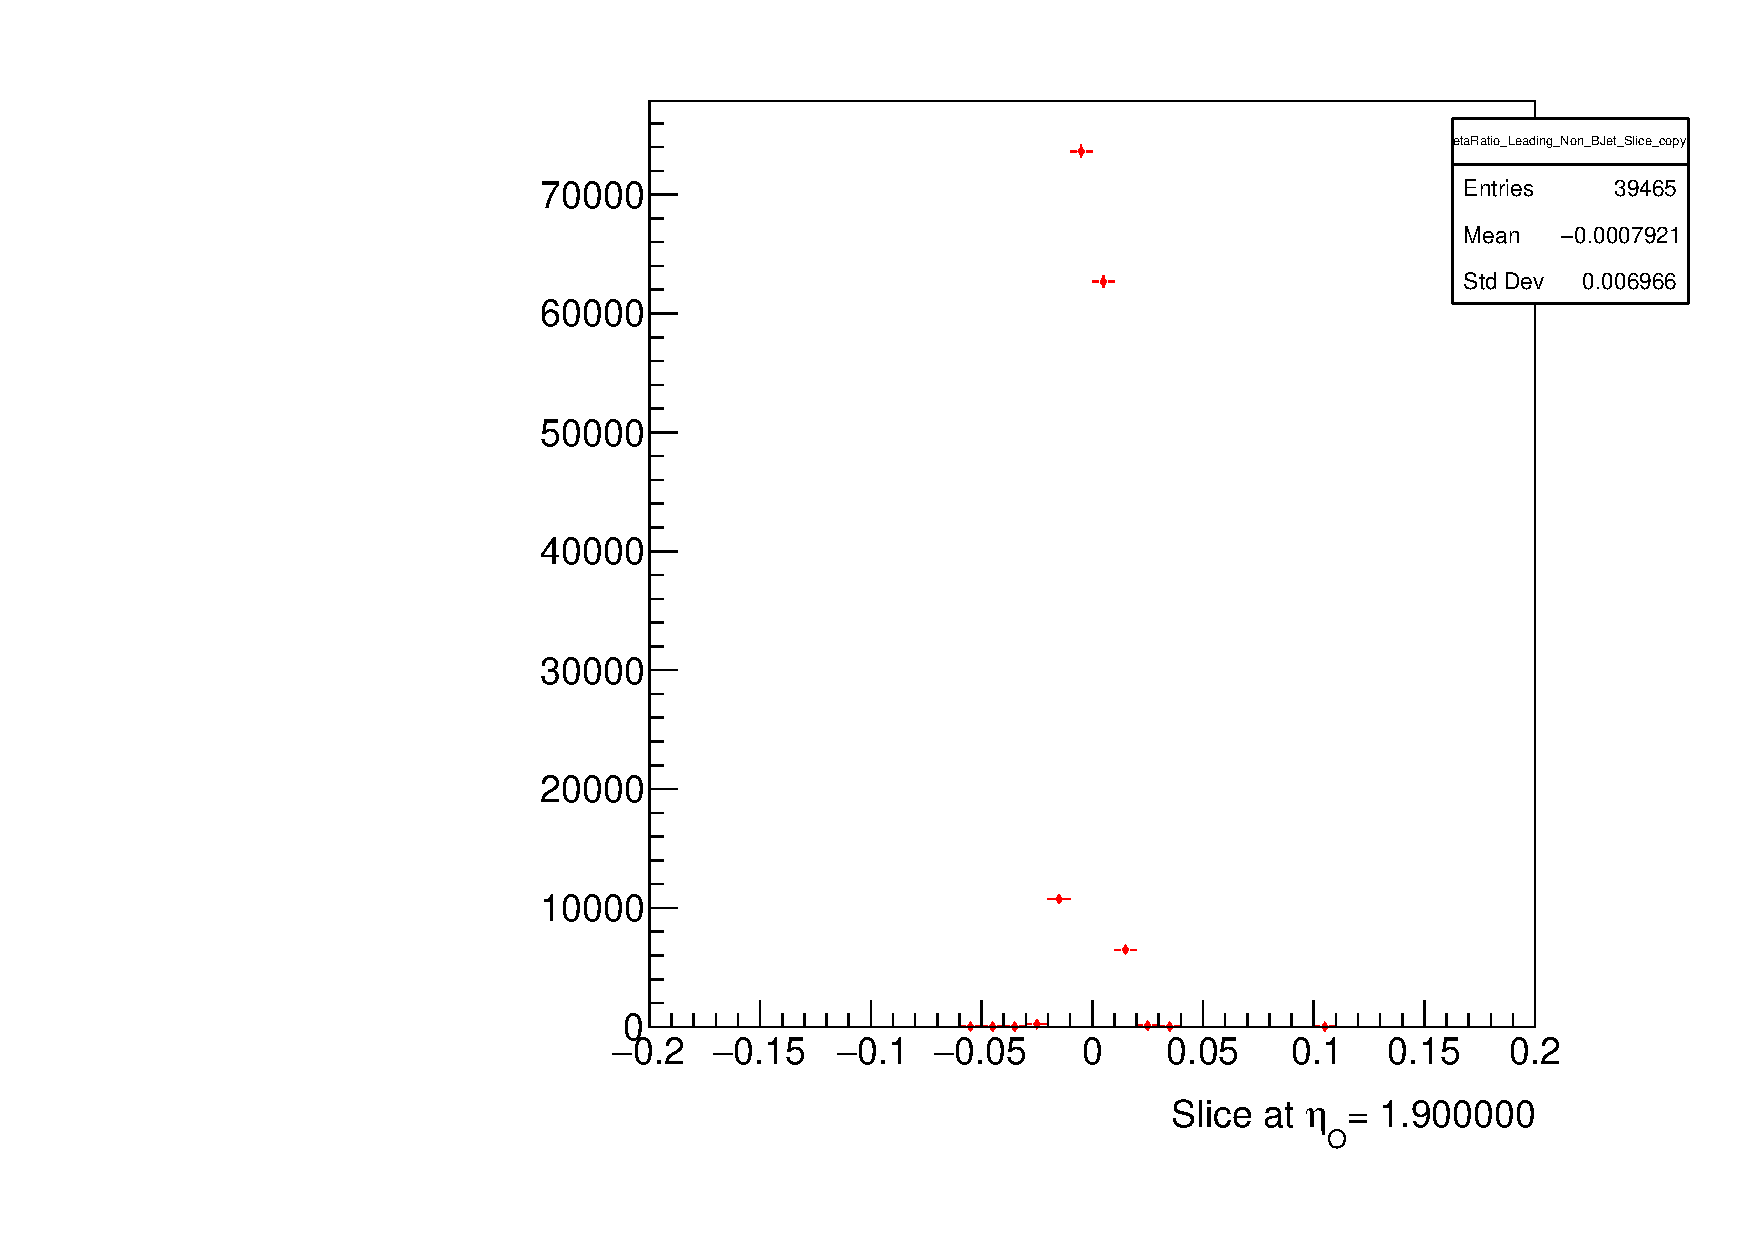
\includegraphics[width=1\linewidth]{etaRatio_Leading_Non_BJet_Slice}
			\end{minipage}
			\caption{$\Delta \eta_{ratio}$ for the leading \pt non $b$-jet from MC events against $\eta$ of the offline $b$-jet. A slice across the $y$-axis has been taken at $\eta=-1.9$. }
			\label{fig:MC:nonleadingbeta}
		\end{figure}
		
		\begin{figure}[h]
			\centering
			
			\begin{minipage}[h]{0.33\linewidth}
				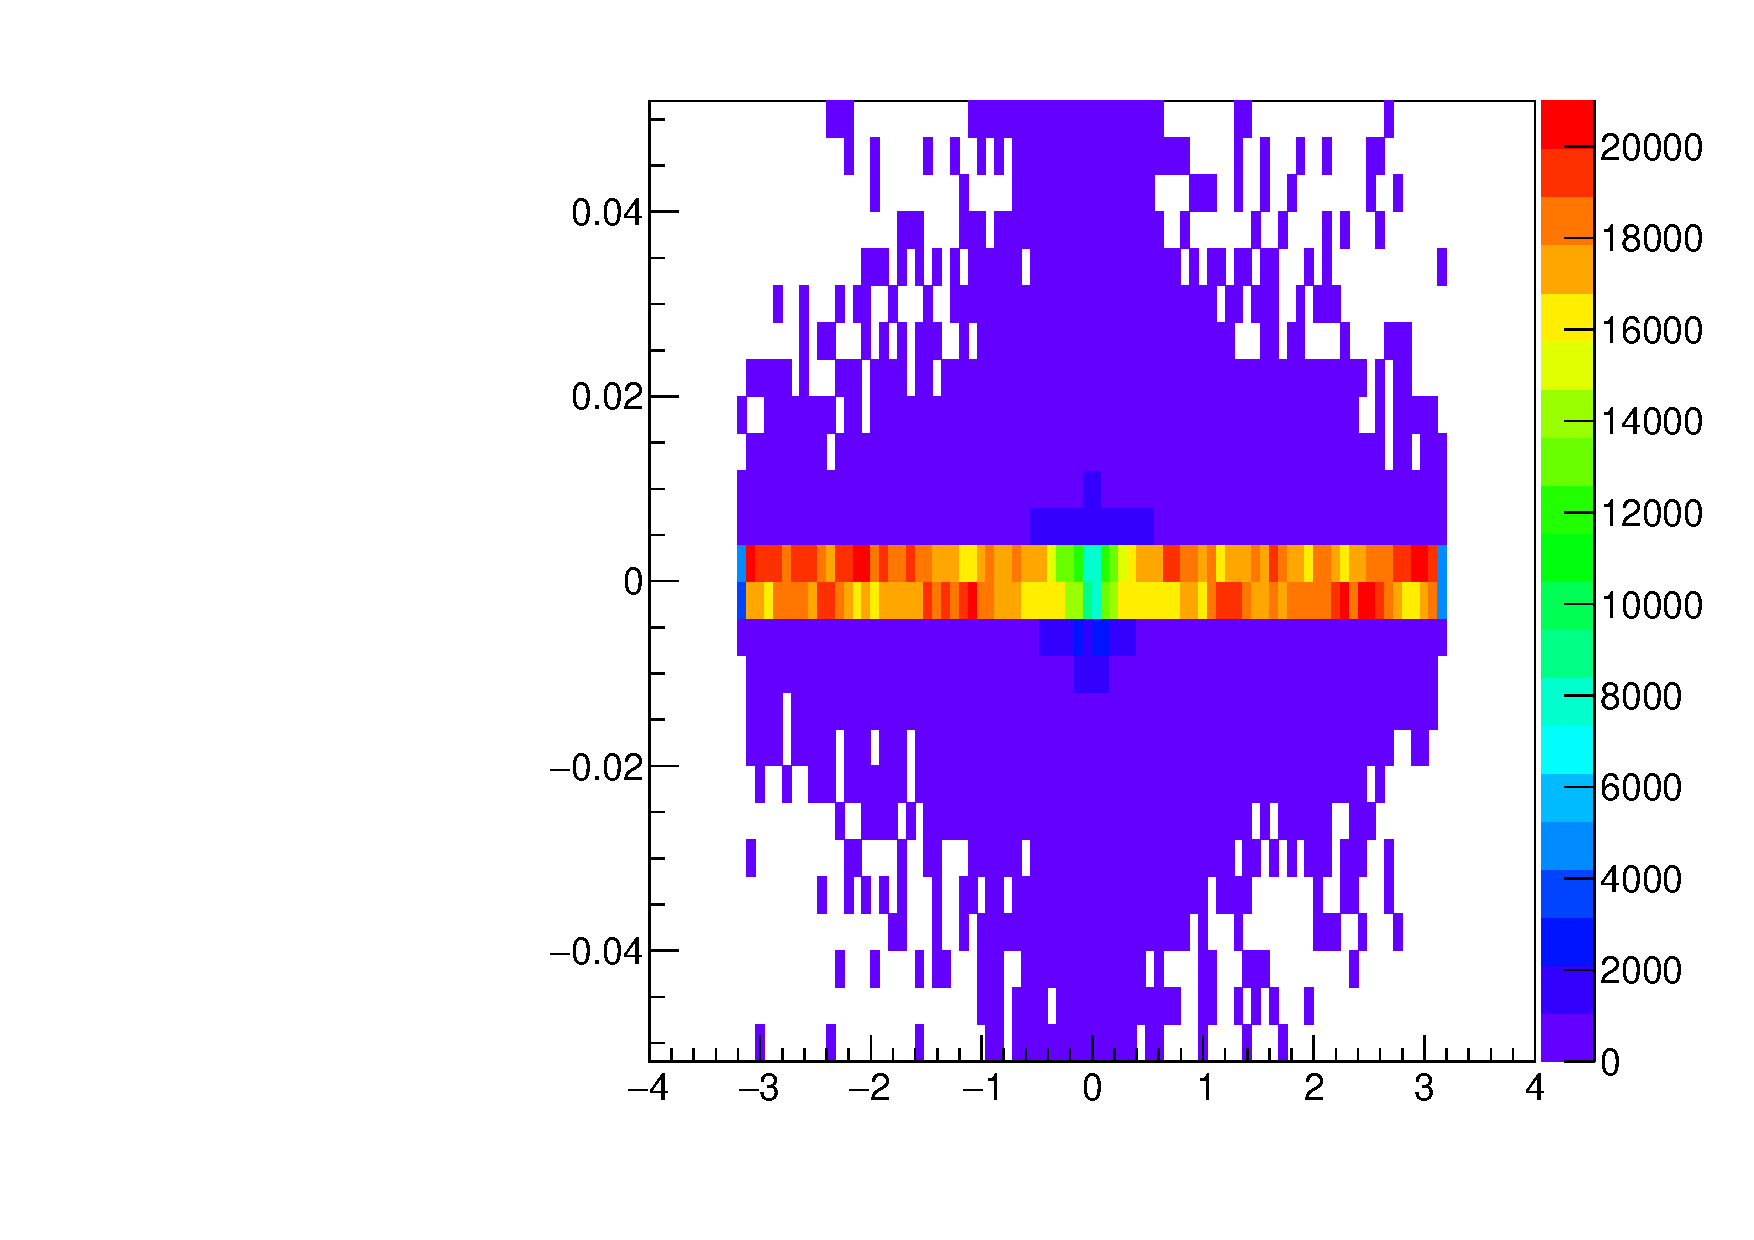
\includegraphics[width=1\linewidth]{phiRatio_Leading_Non_BJet}
			\end{minipage}
			\quad
			\begin{minipage}[h]{0.33\linewidth}
				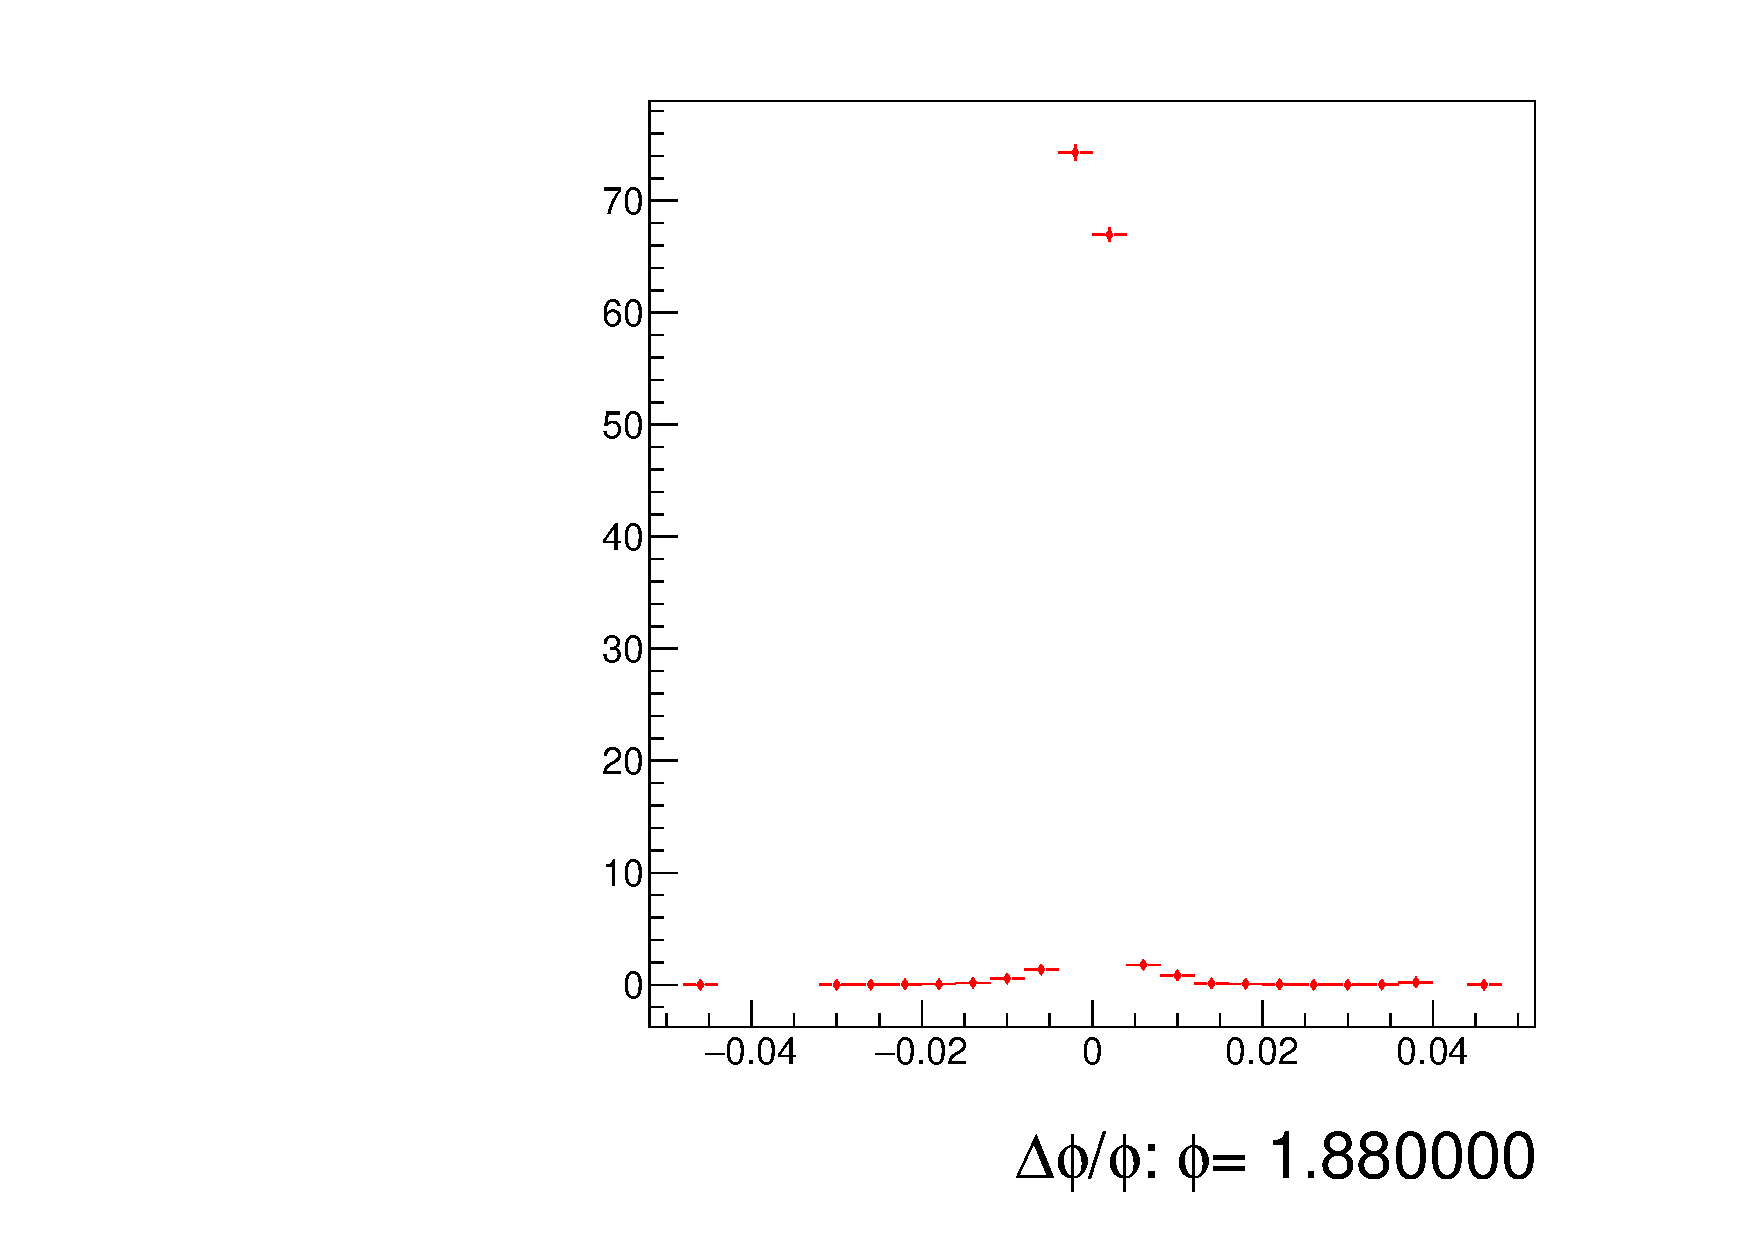
\includegraphics[width=1\linewidth]{phiRatio_Leading_Non_BJet_Slice}
			\end{minipage}
			\caption{$\Delta \phi_{ratio}$ for the leading \pt non $b$-jet from MC events against $\phi$ of the offline $b$-jet. A slice across the $y$-axis has been taken at $\phi=-1.64$. }
			\label{fig:MC:nonleadingbphi}
		\end{figure}
		
		\begin{figure}[h]
			\centering
			
			\begin{minipage}[h]{0.33\linewidth}
				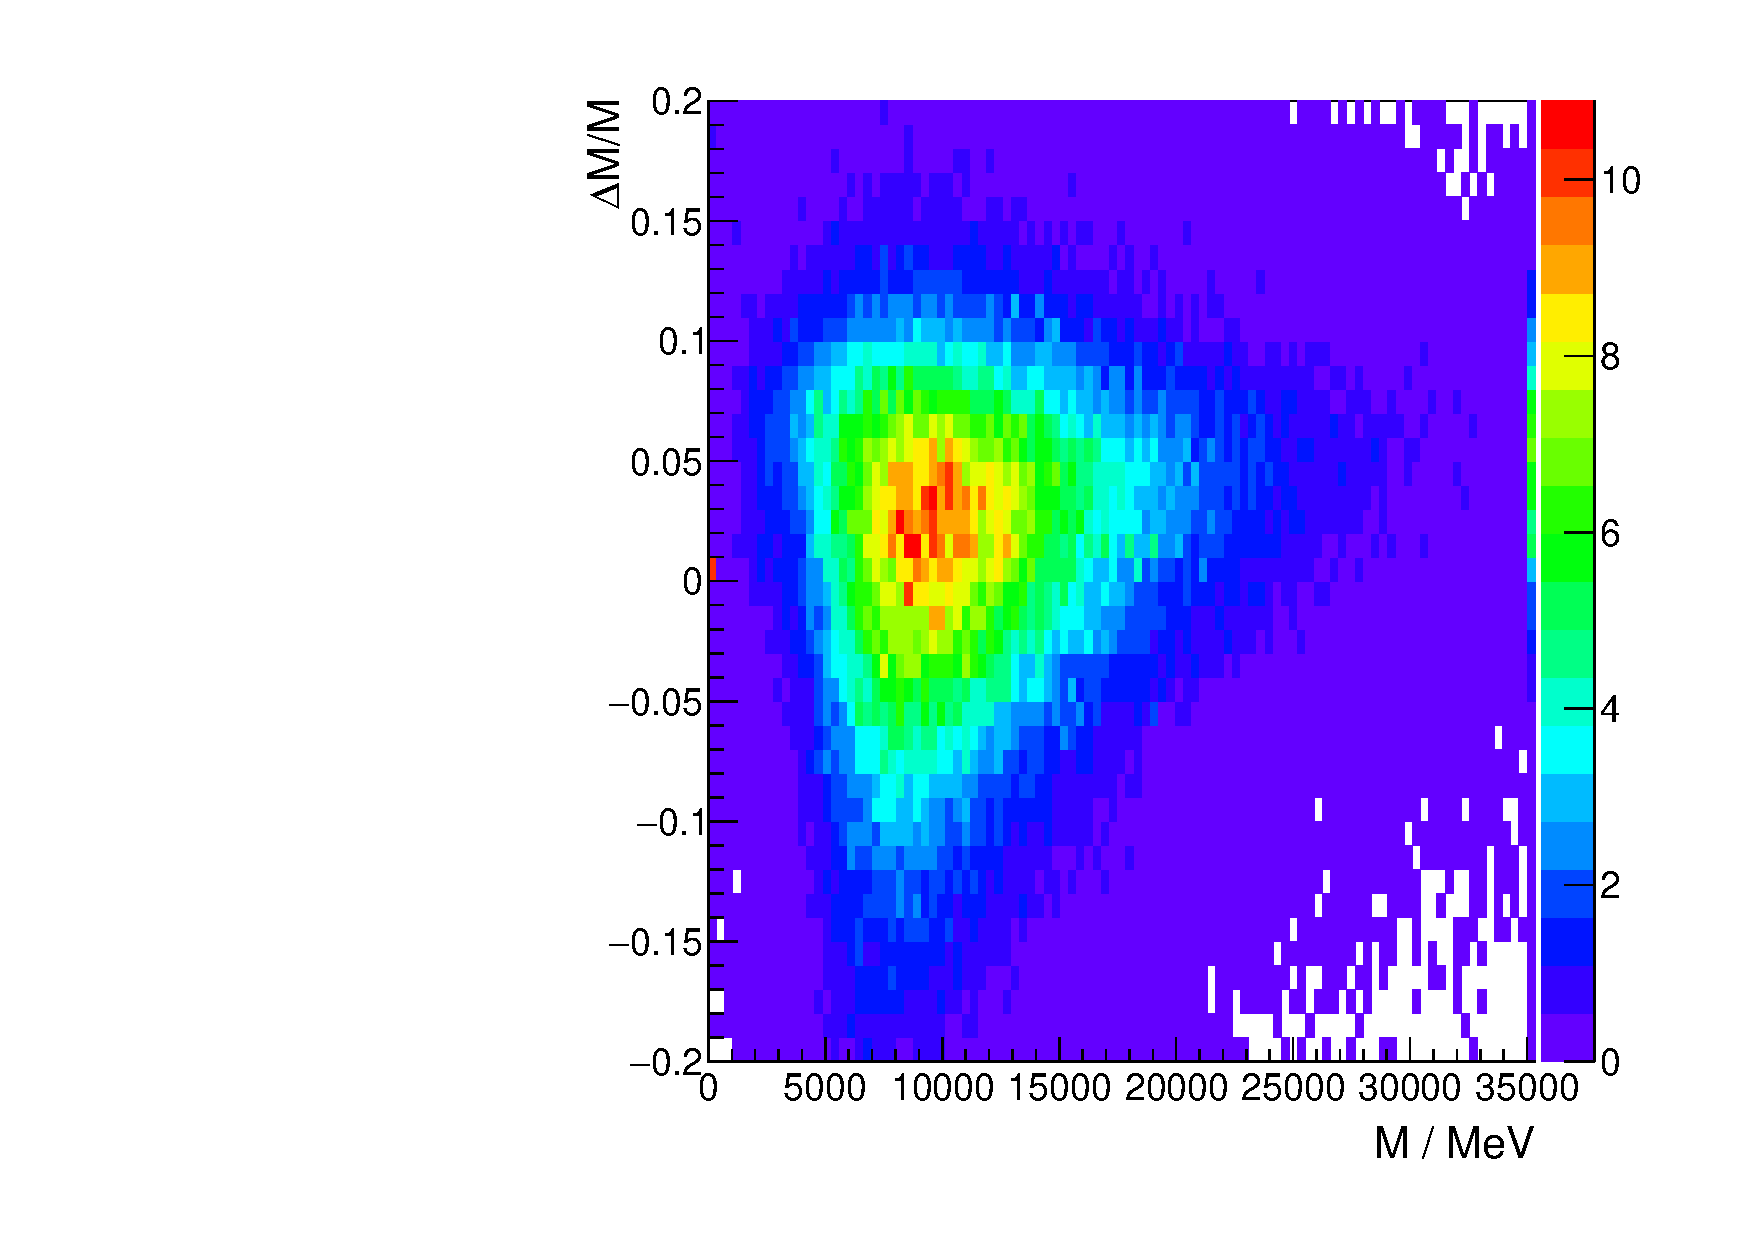
\includegraphics[width=1\linewidth]{mRatio_Leading_Non_BJet}
			\end{minipage}
			\quad
			\begin{minipage}[h]{0.33\linewidth}
				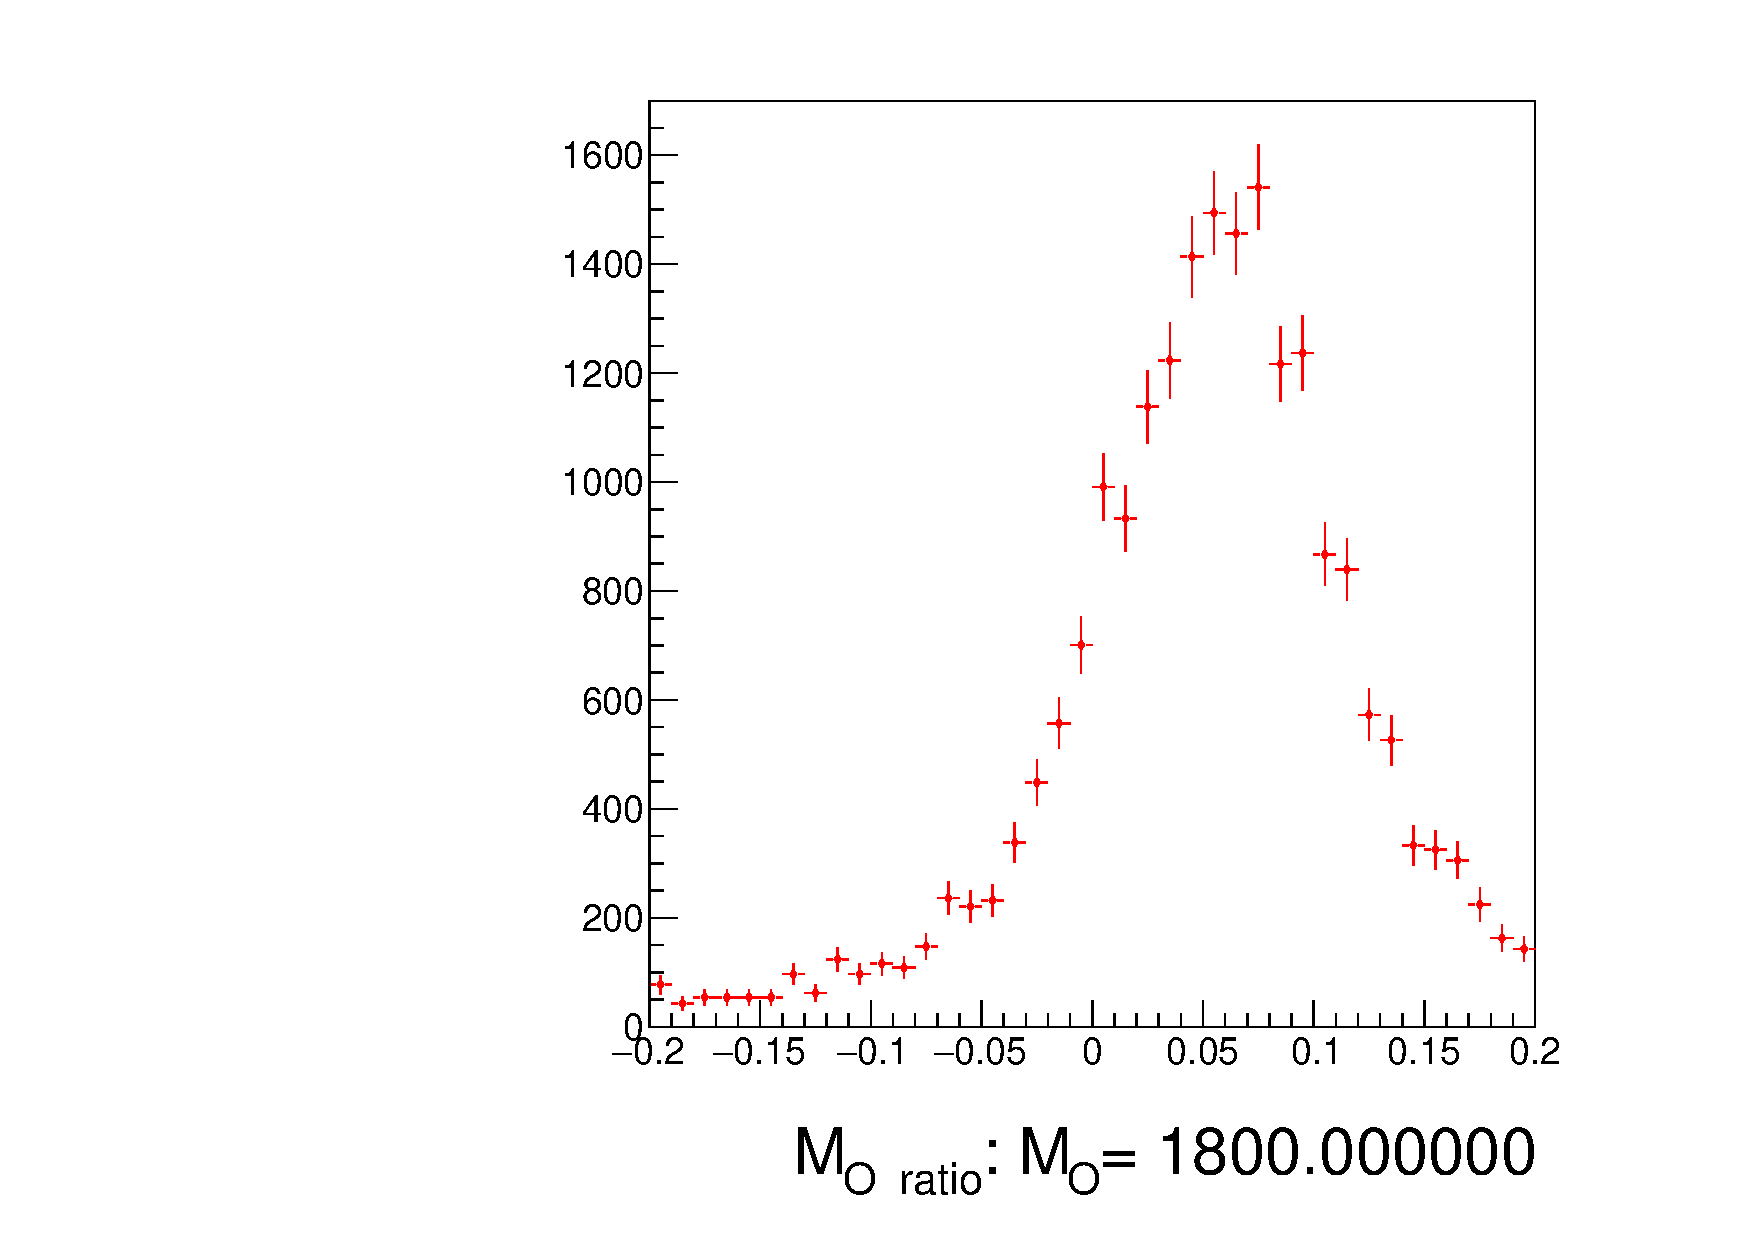
\includegraphics[width=1\linewidth]{mRatio_Leading_Non_BJet_Slice}
			\end{minipage}
			\caption{$\Delta M_{ratio}$ for the leading \pt non $b$-jet from MC events against $M$ of the offline $b$-jet. A slice across the $y$-axis has been taken at $M=7$GeV. }
			\label{fig:MC:nonleadingbm}
		\end{figure}
	
	\newpage
	\subsection{Data}
	
		\begin{figure}[h]
			\centering
			
			\begin{minipage}[h]{0.33\linewidth}
				
\includegraphics[width=1\linewidth]{placeholder}
				\caption{}
				\label{fig:D:leadingnonbpt}
			\end{minipage}
			\quad
			\begin{minipage}[h]{0.33\linewidth}
				
\includegraphics[width=1\linewidth]{placeholder}
				\caption{}
				\label{fig:D:leadingnonbeta}
			\end{minipage}
		\end{figure}
		
		\begin{figure}[h]
			\centering
			
			\begin{minipage}[h]{0.33\linewidth}
				
\includegraphics[width=1\linewidth]{placeholder}
				\caption{}
				\label{fig:D:leadingnonbphi}
			\end{minipage}
			\quad
			\begin{minipage}[h]{0.33\linewidth}
				
\includegraphics[width=1\linewidth]{placeholder}
				\caption{}
				\label{fig:D:leadingnonbm}
			\end{minipage}
		\end{figure}
		
		\newpage
\section{Central Jets}

\section{Forward Jets}

\section{Extremal?  Jets}

\section{Jet Tagging Efficiency}

	As covered in Section \ref{det:btaggingdiff}, the differences between the $b$-tagging methods for online and offline necessitates a comparison between the tagging efficiencies. This comparison could only be carried out on the MC, as the truth label of the offline jet was required to categorise each pair.
	
	\newpage
	\subsection{\textit{b}-jet efficiency} 
	
		\begin{figure}[h]
			\centering
			\begin{minipage}[h]{0.31\linewidth}
				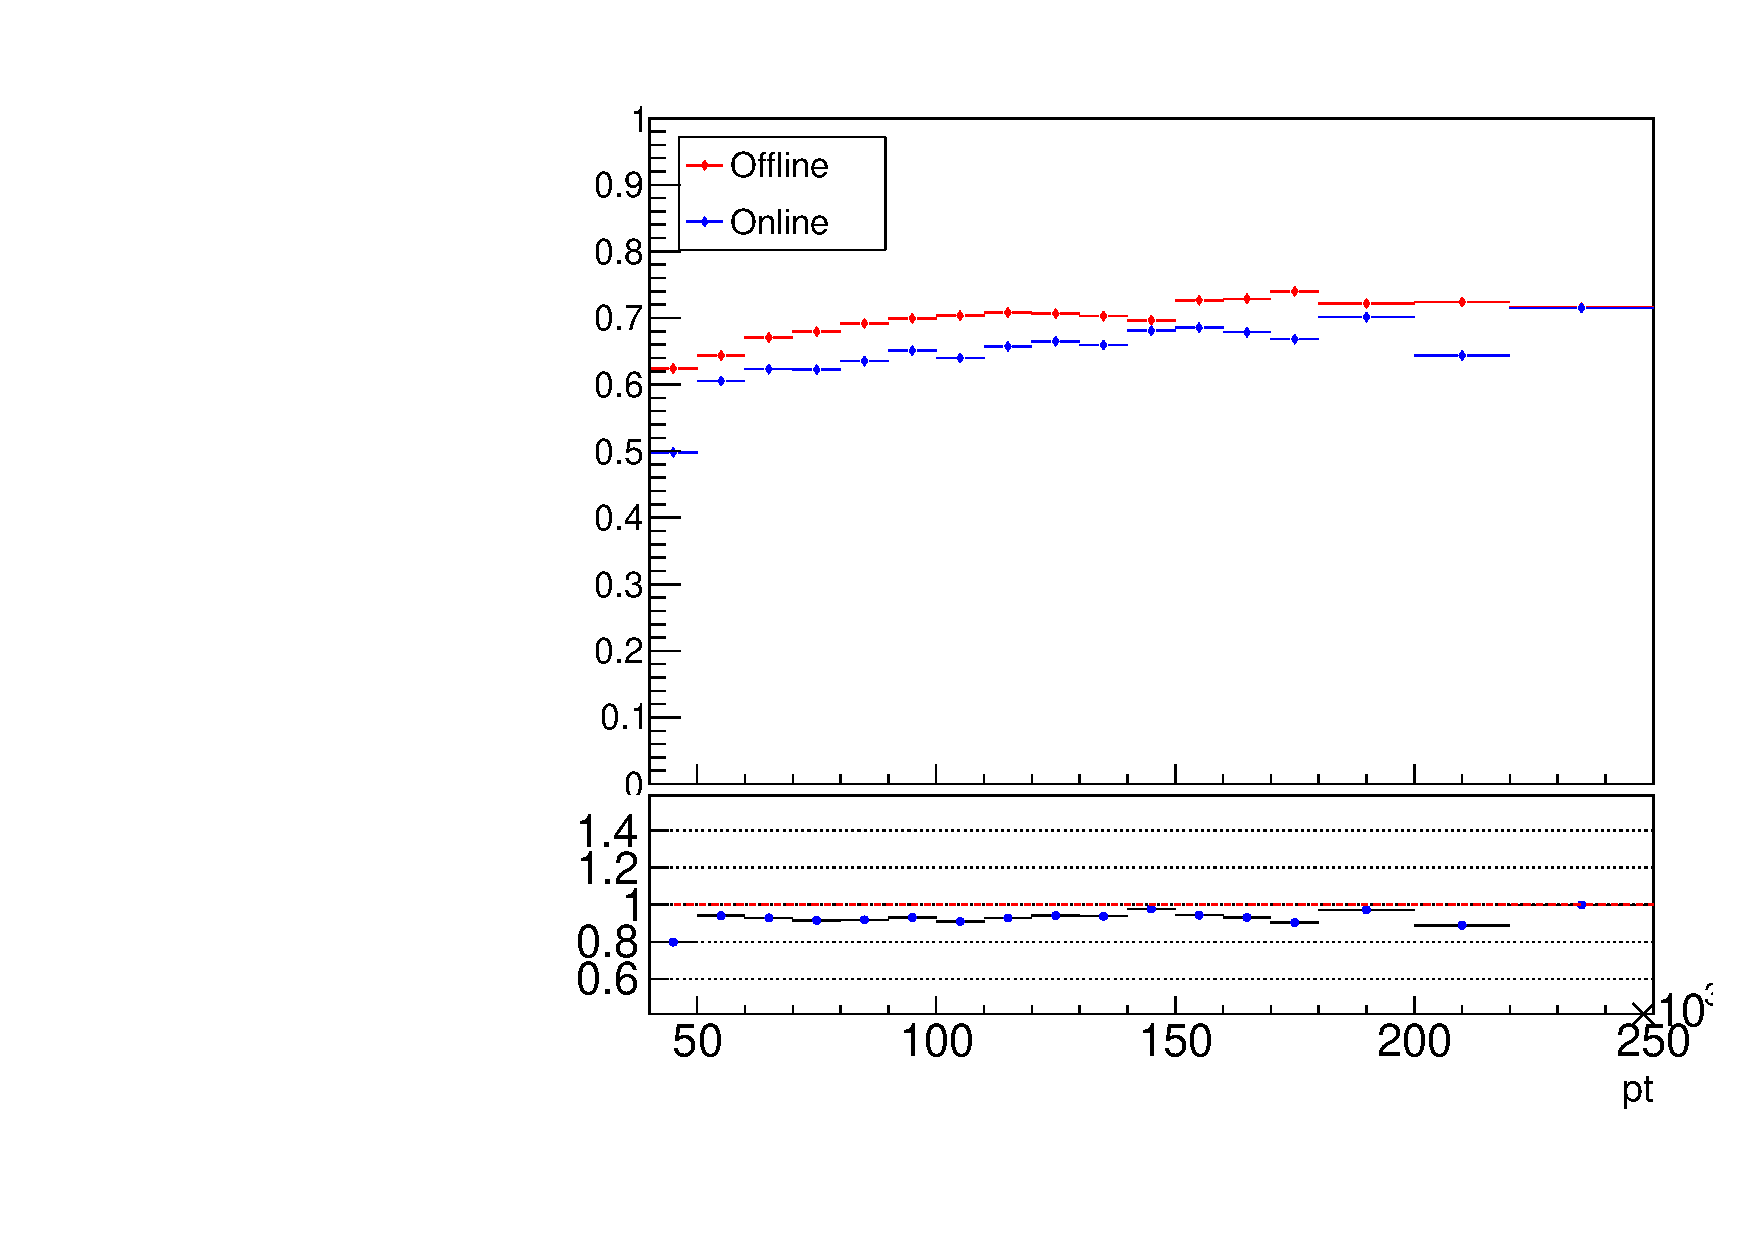
\includegraphics[width=1\linewidth]{ptBJET}
				
			\end{minipage}
			\quad
			\begin{minipage}[h]{0.31\linewidth}
				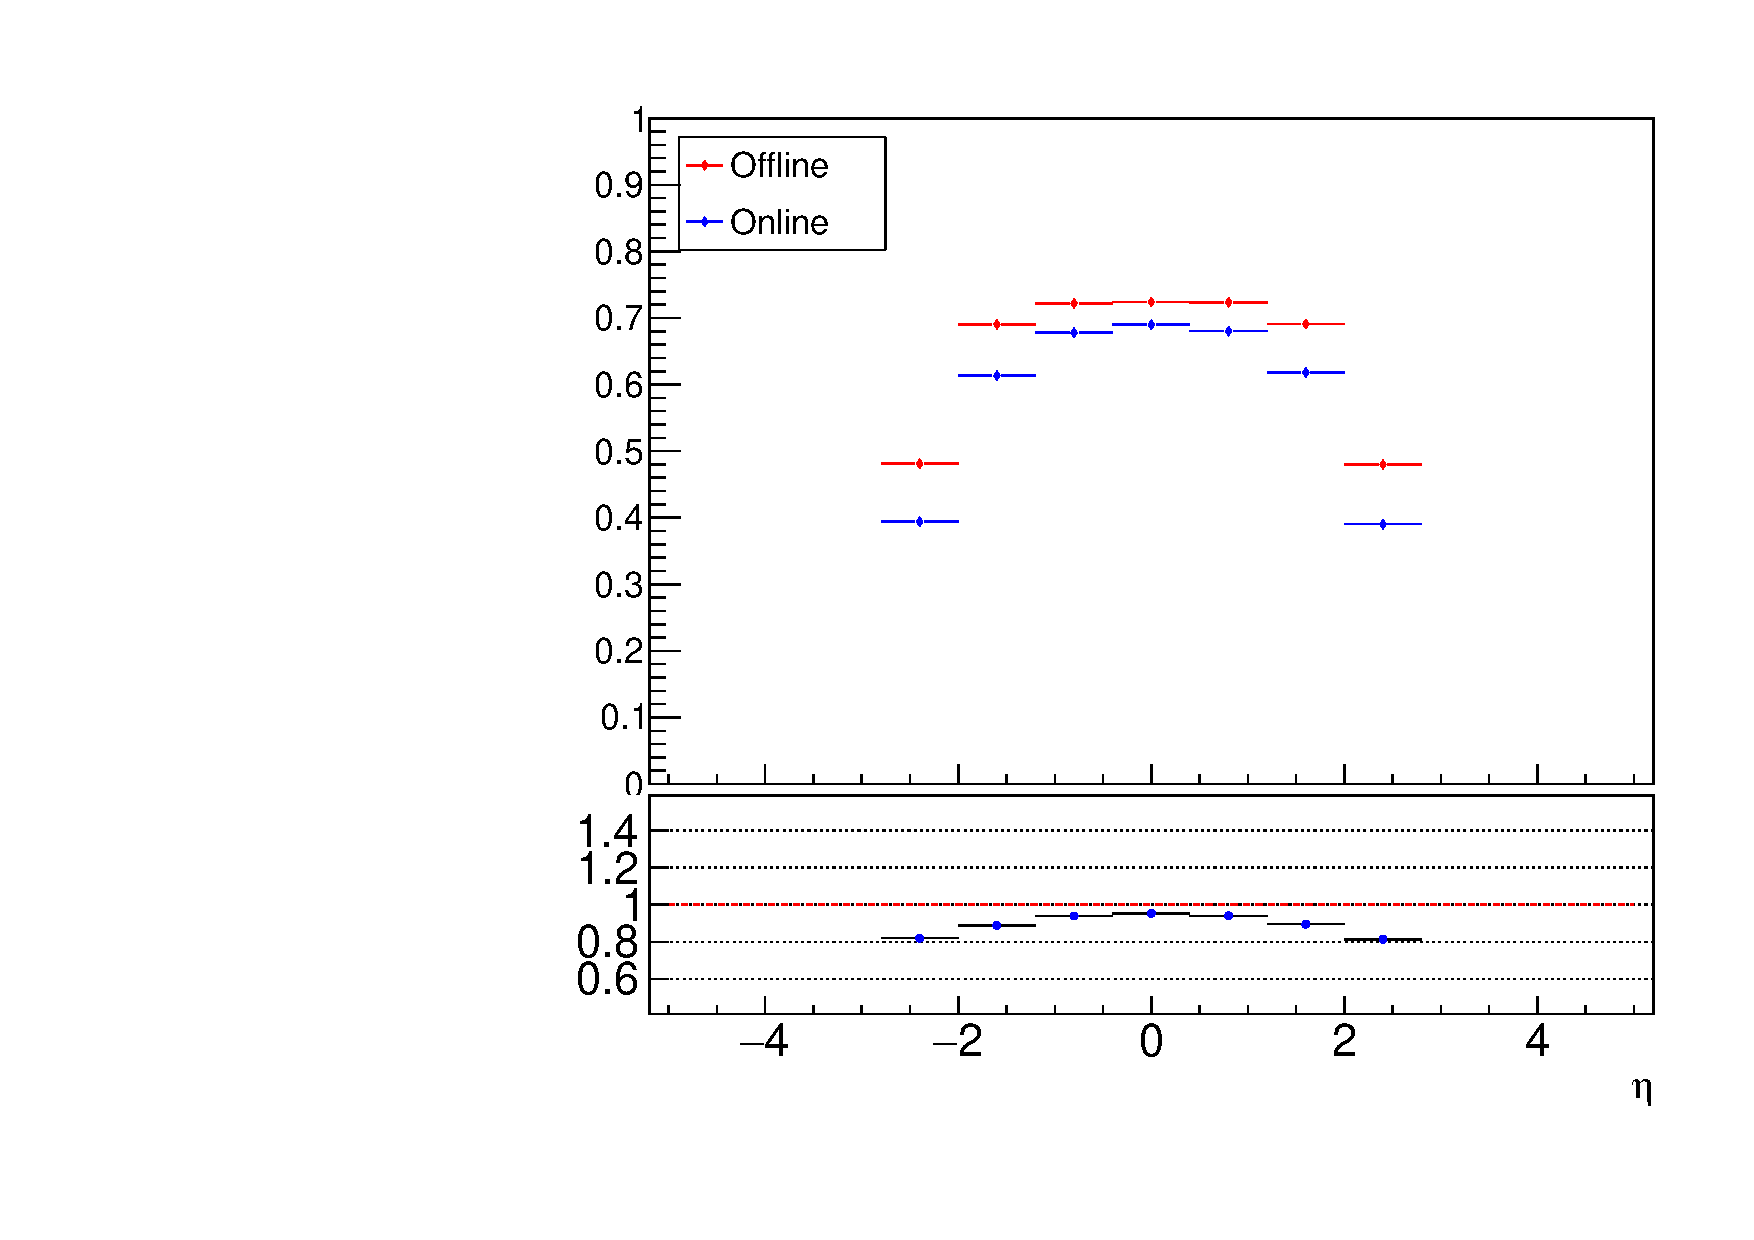
\includegraphics[width=1\linewidth]{etaBJET}
			\end{minipage}
			\quad
			\begin{minipage}[h]{0.31\linewidth}
				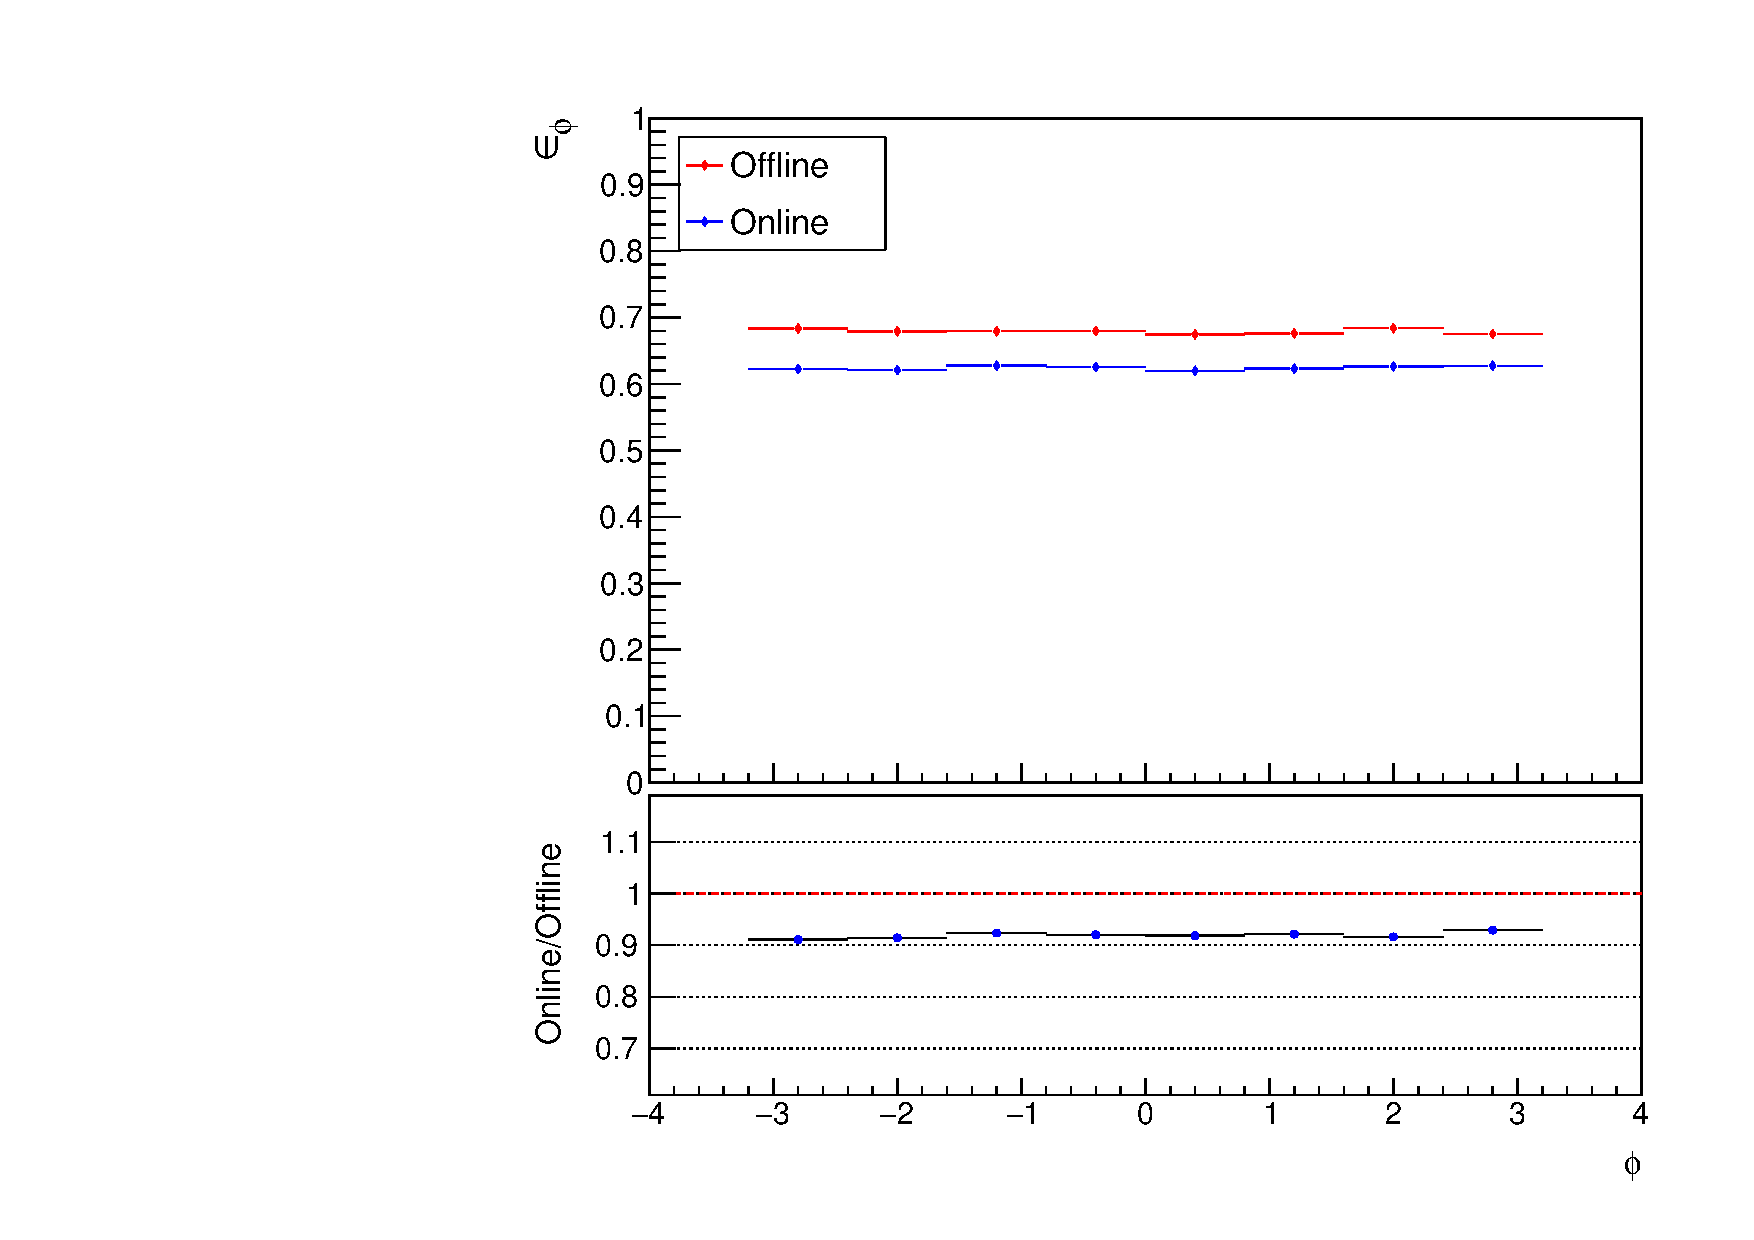
\includegraphics[width=1\linewidth]{phiBJET}
			\end{minipage}
			\caption{ }
			\label{fig:MC:bjetefficiency}
		\end{figure}
			
			\todo{Options, could show more vars or alternatively the reference hists, or alternatively just reference the references}
	
	\subsection{\textit{c}-jet efficiency} 
	
		\begin{figure}[h]
			\centering
			\begin{minipage}[h]{0.31\linewidth}
				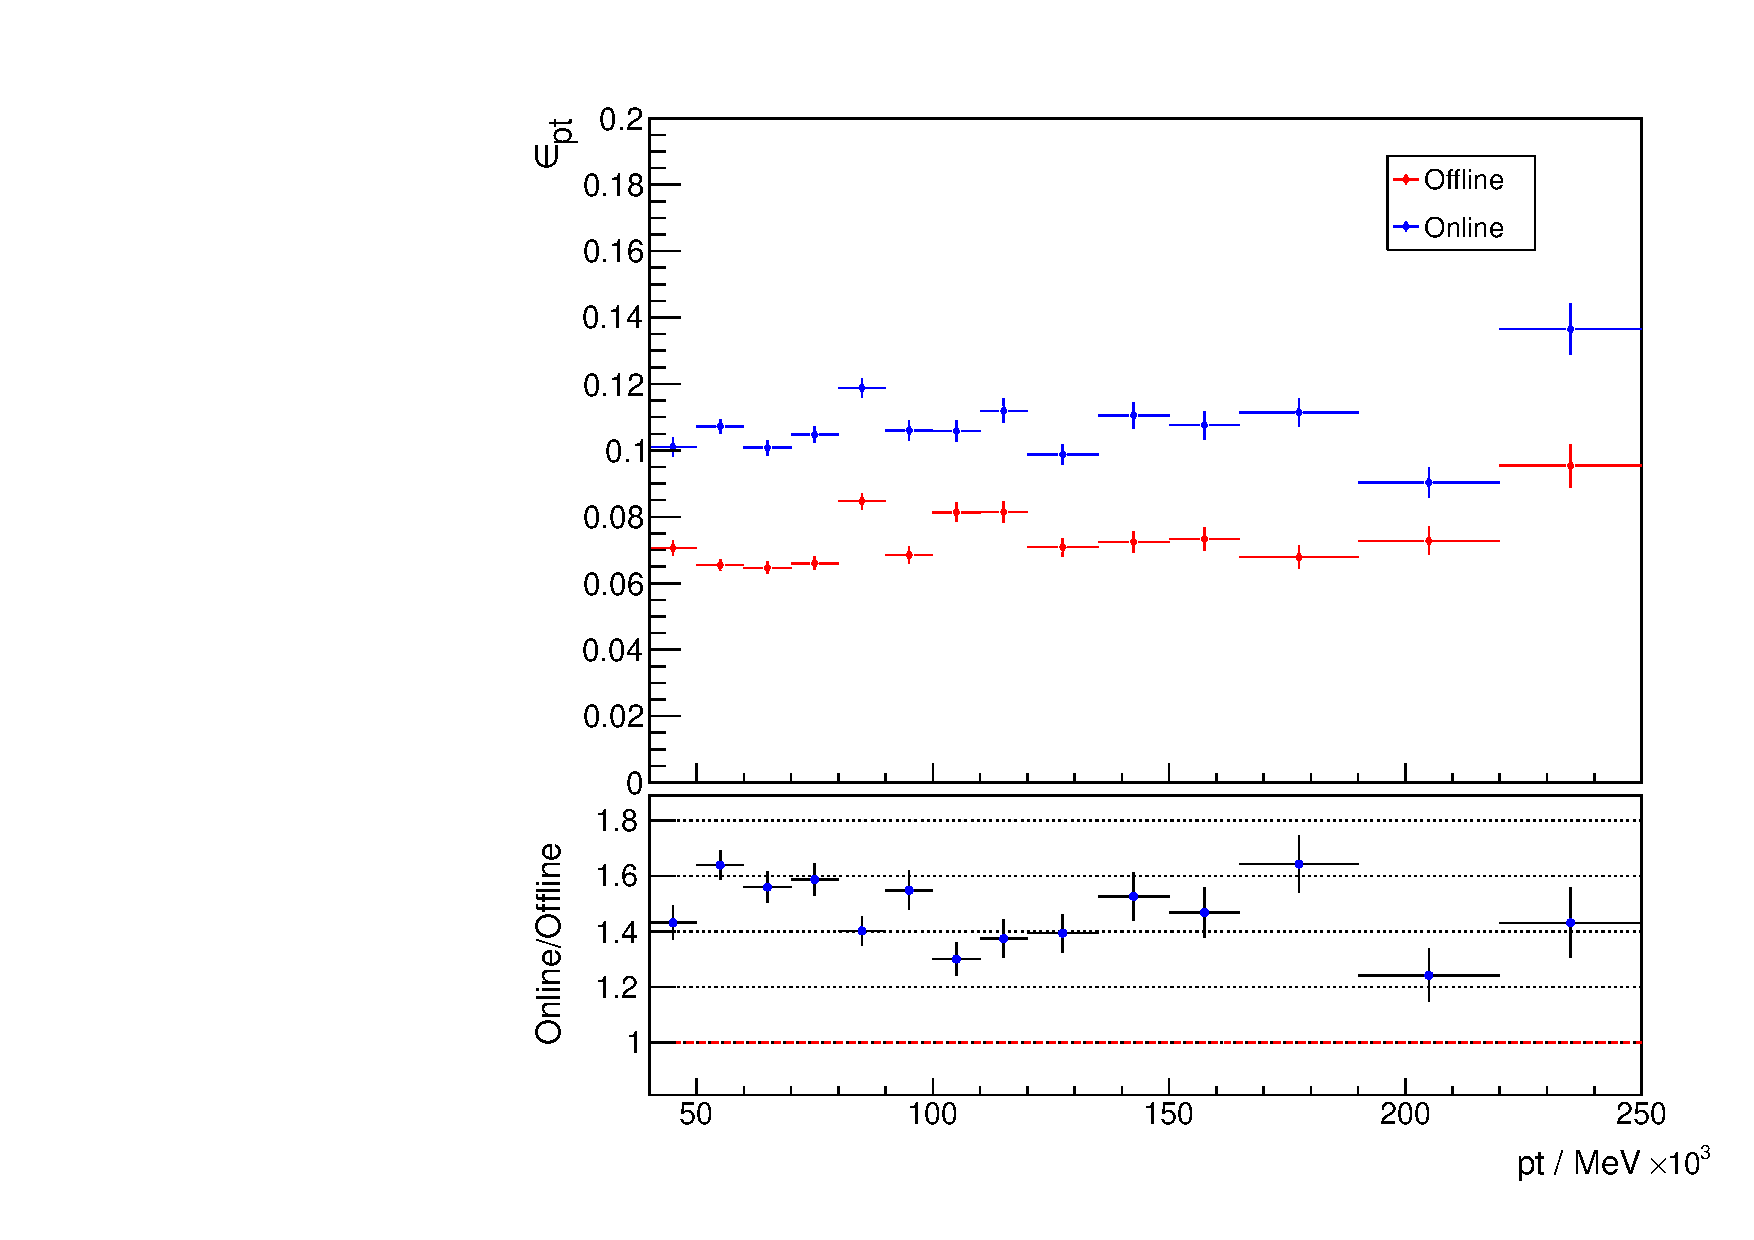
\includegraphics[width=1\linewidth]{ptCJET}
				
			\end{minipage}
			\quad
			\begin{minipage}[h]{0.31\linewidth}
				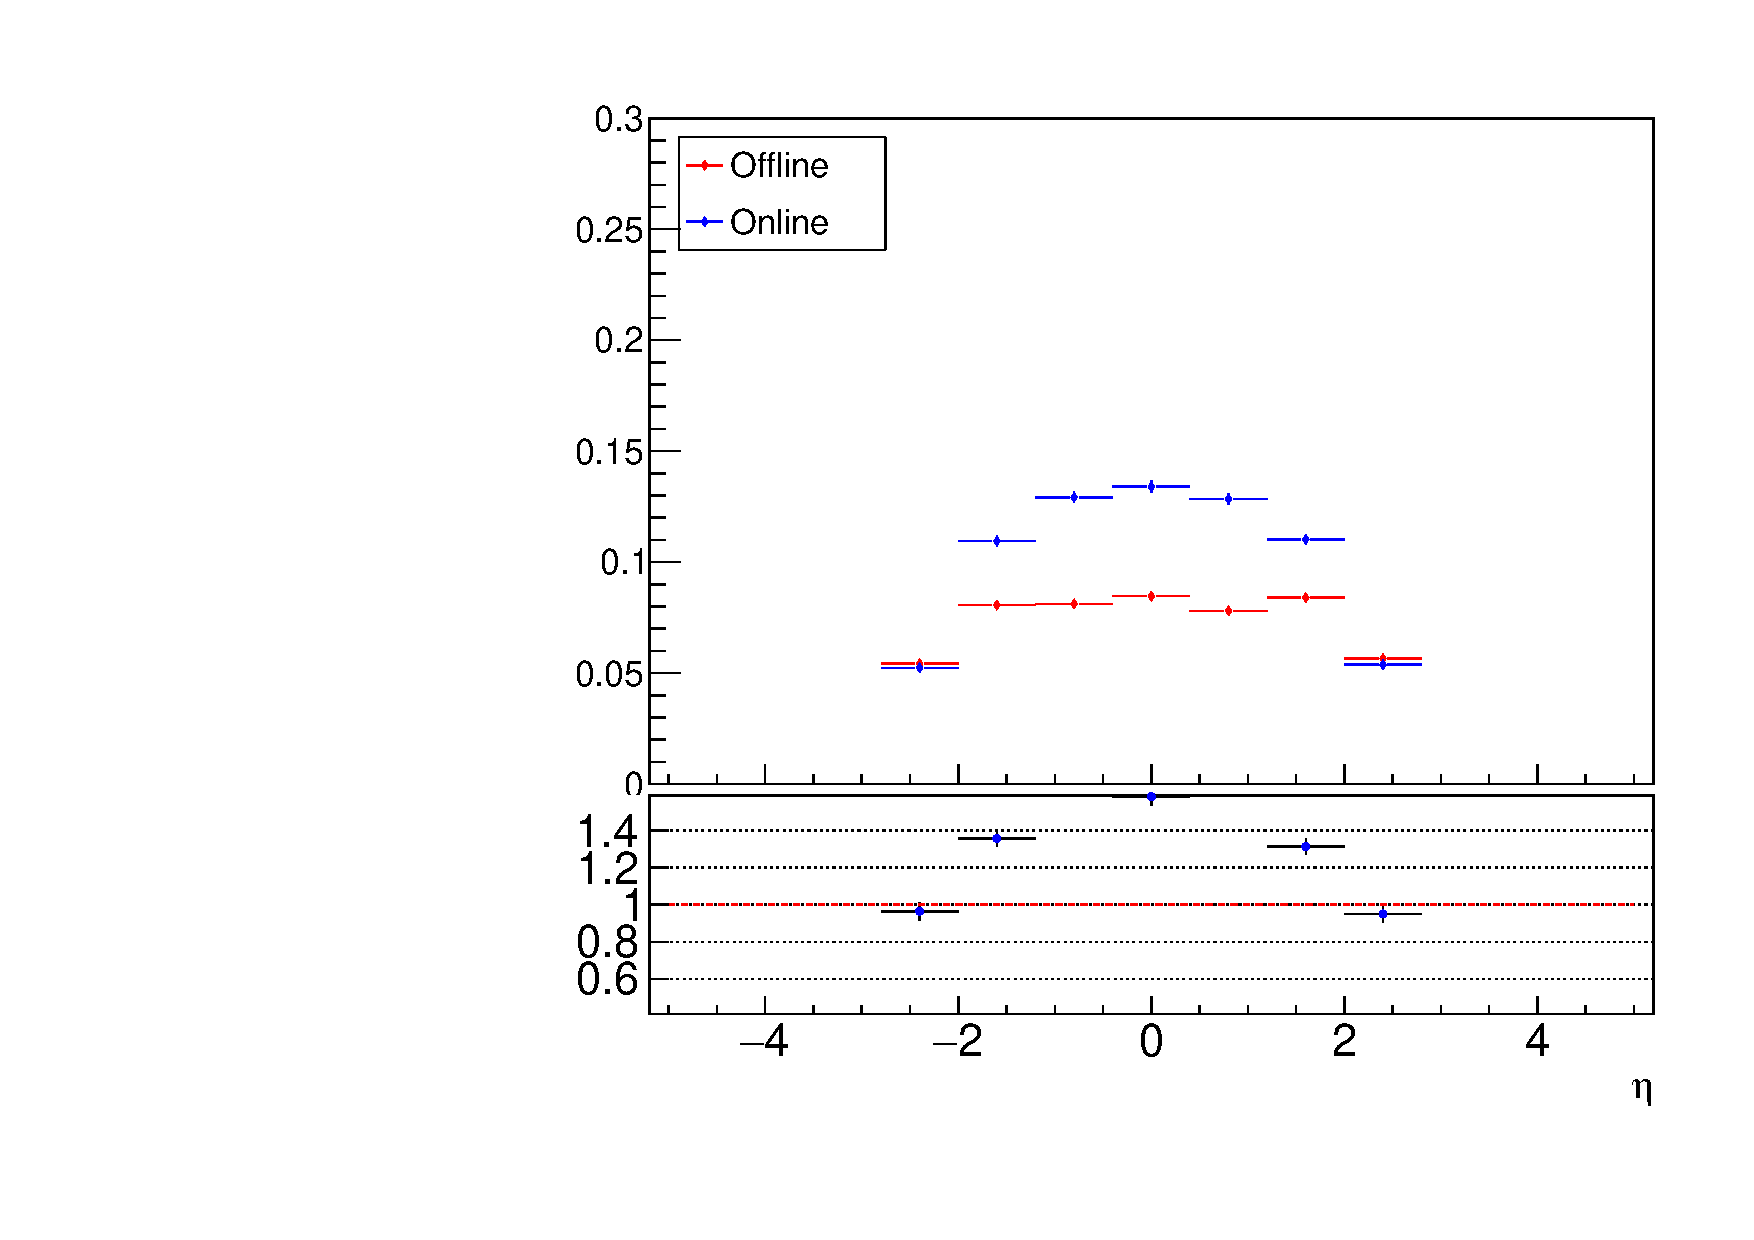
\includegraphics[width=1\linewidth]{etaCJET}
			\end{minipage}
			\quad
			\begin{minipage}[h]{0.31\linewidth}
				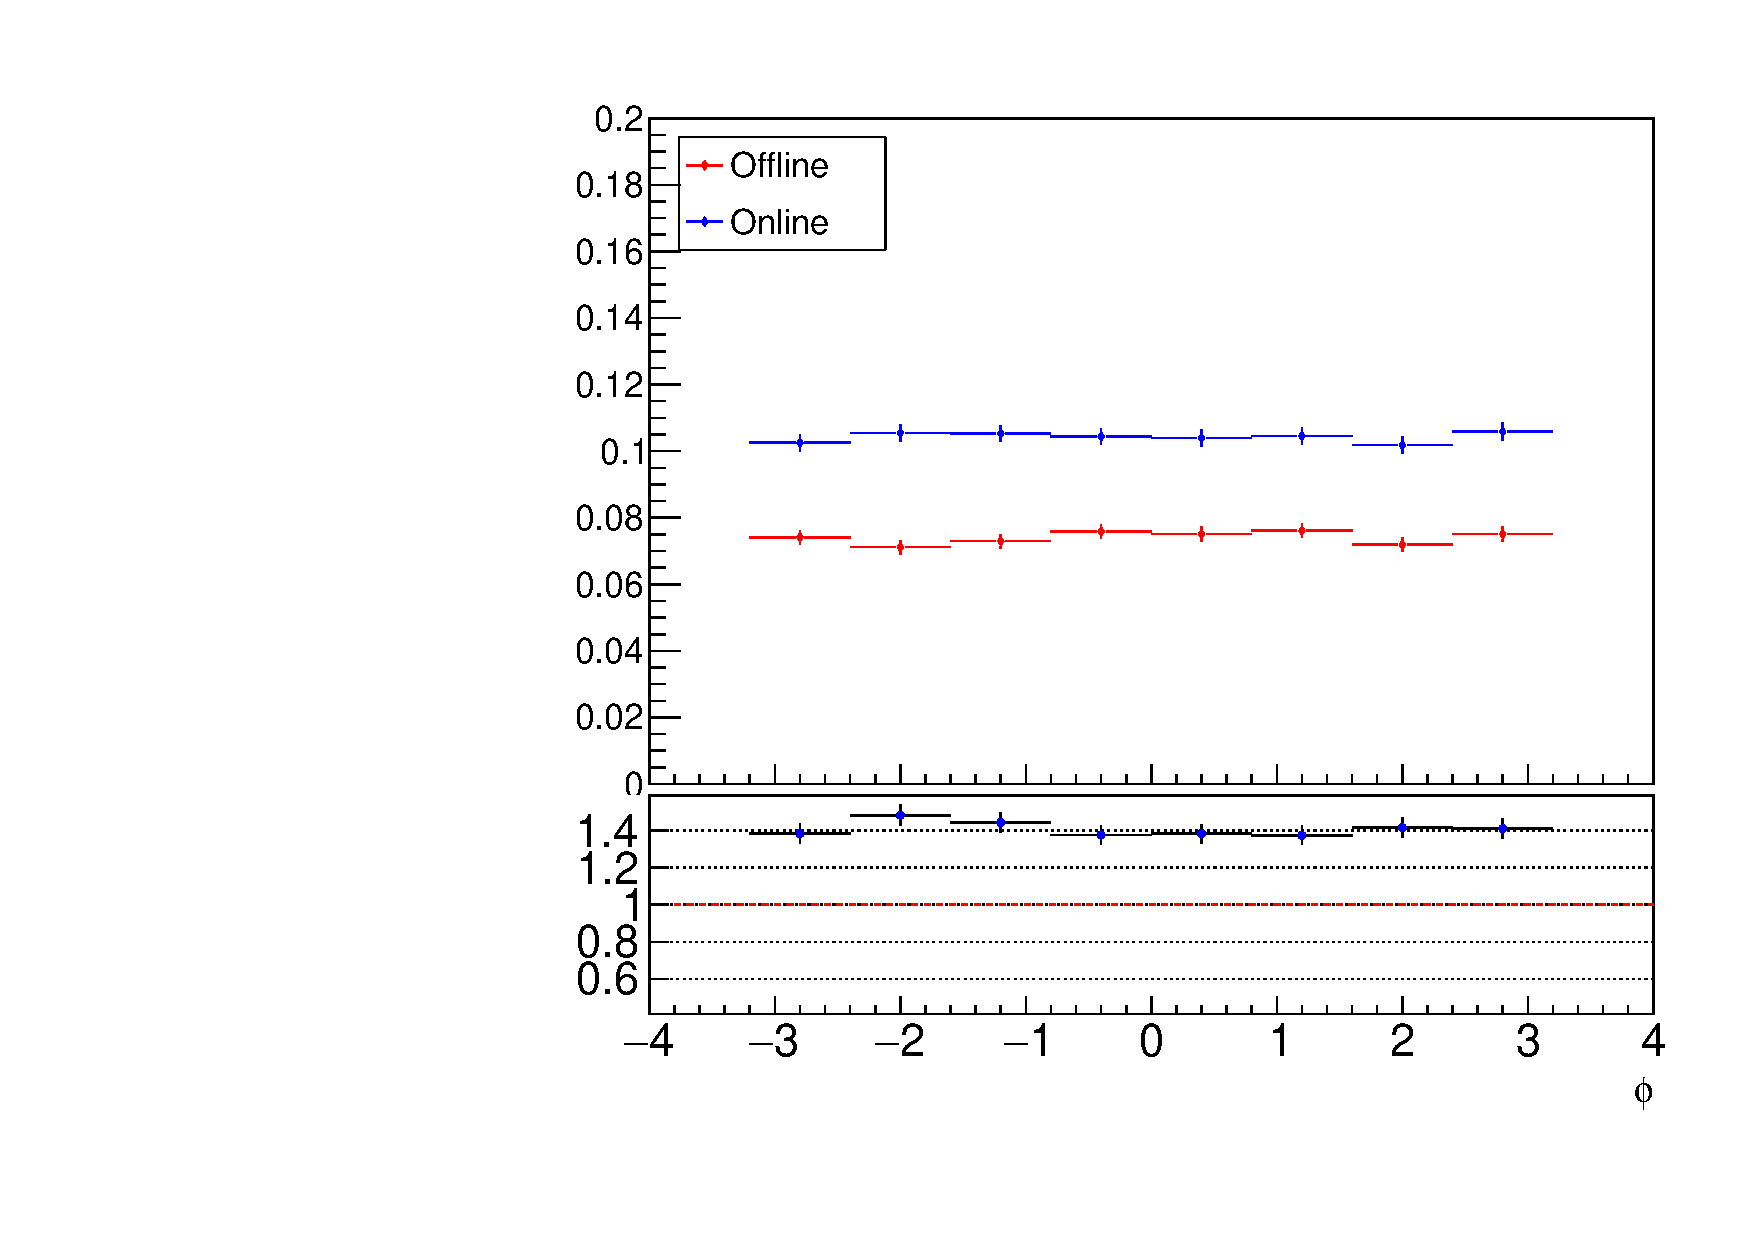
\includegraphics[width=1\linewidth]{phiCJET}
			\end{minipage}
			\caption{ }
			\label{fig:MC:cjetefficiency}
		\end{figure}
	
	\newpage
	\subsection{Light-jet efficiency}
	
		\begin{figure}[h]
			\centering
			\begin{minipage}[h]{0.31\linewidth}
				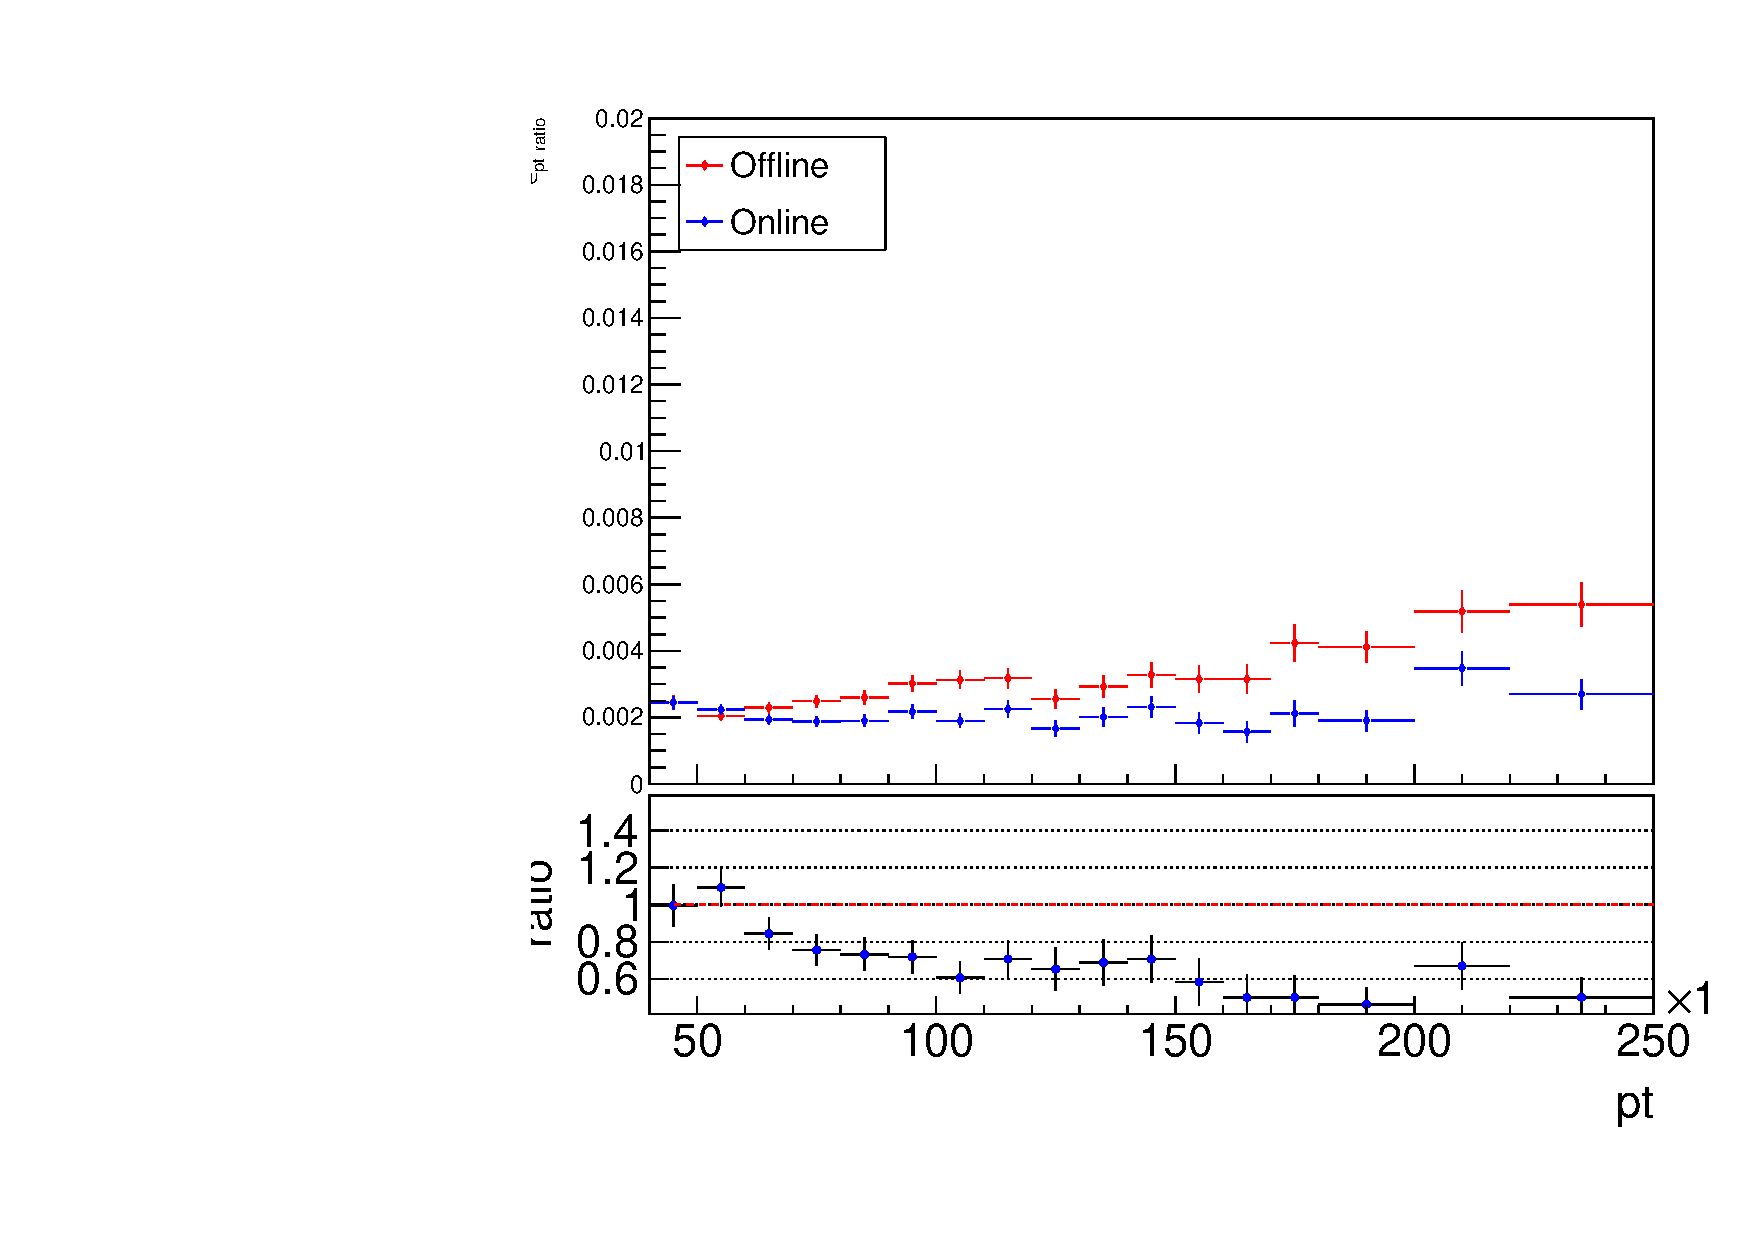
\includegraphics[width=1\linewidth]{ptLIGHTJET}
				
			\end{minipage}
			\quad
			\begin{minipage}[h]{0.31\linewidth}
				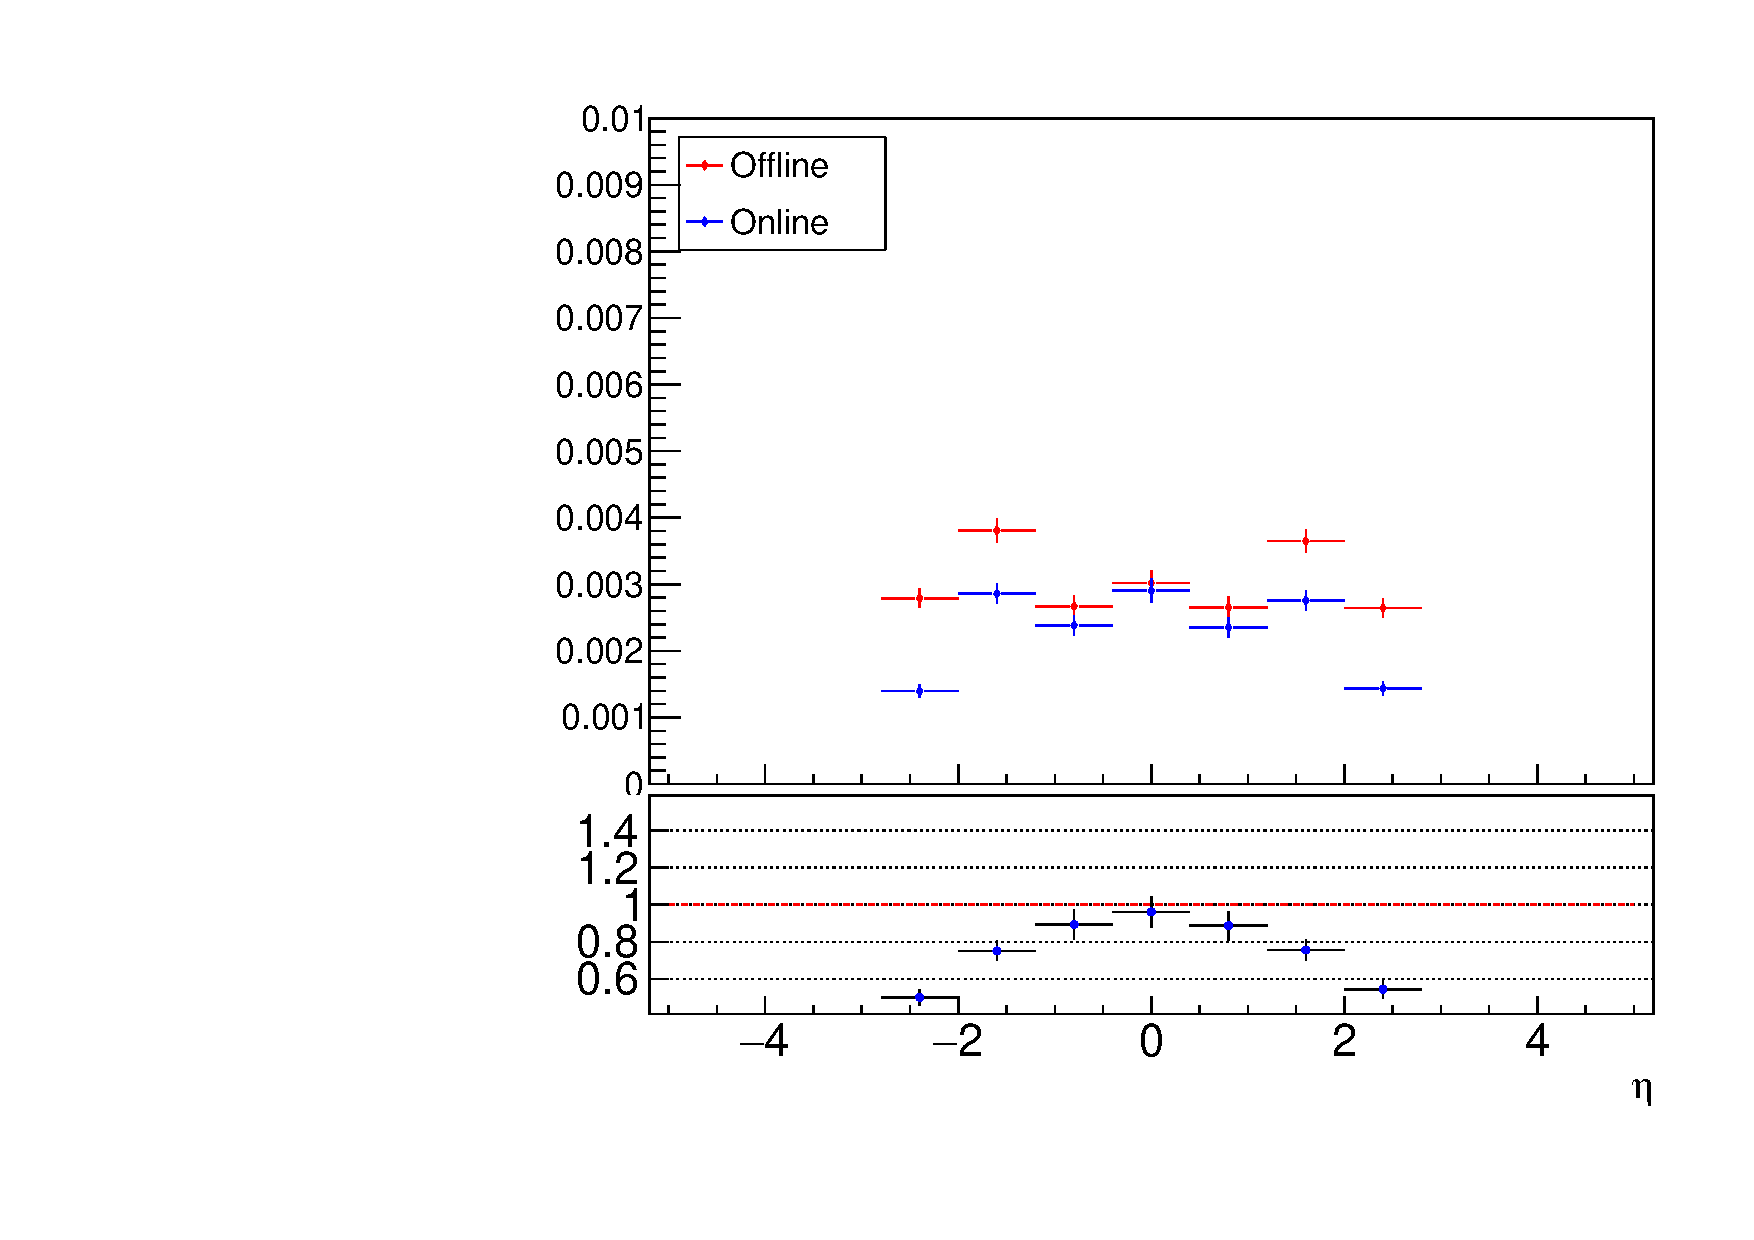
\includegraphics[width=1\linewidth]{etaLIGHTJET}
			\end{minipage}
			\quad
			\begin{minipage}[h]{0.31\linewidth}
				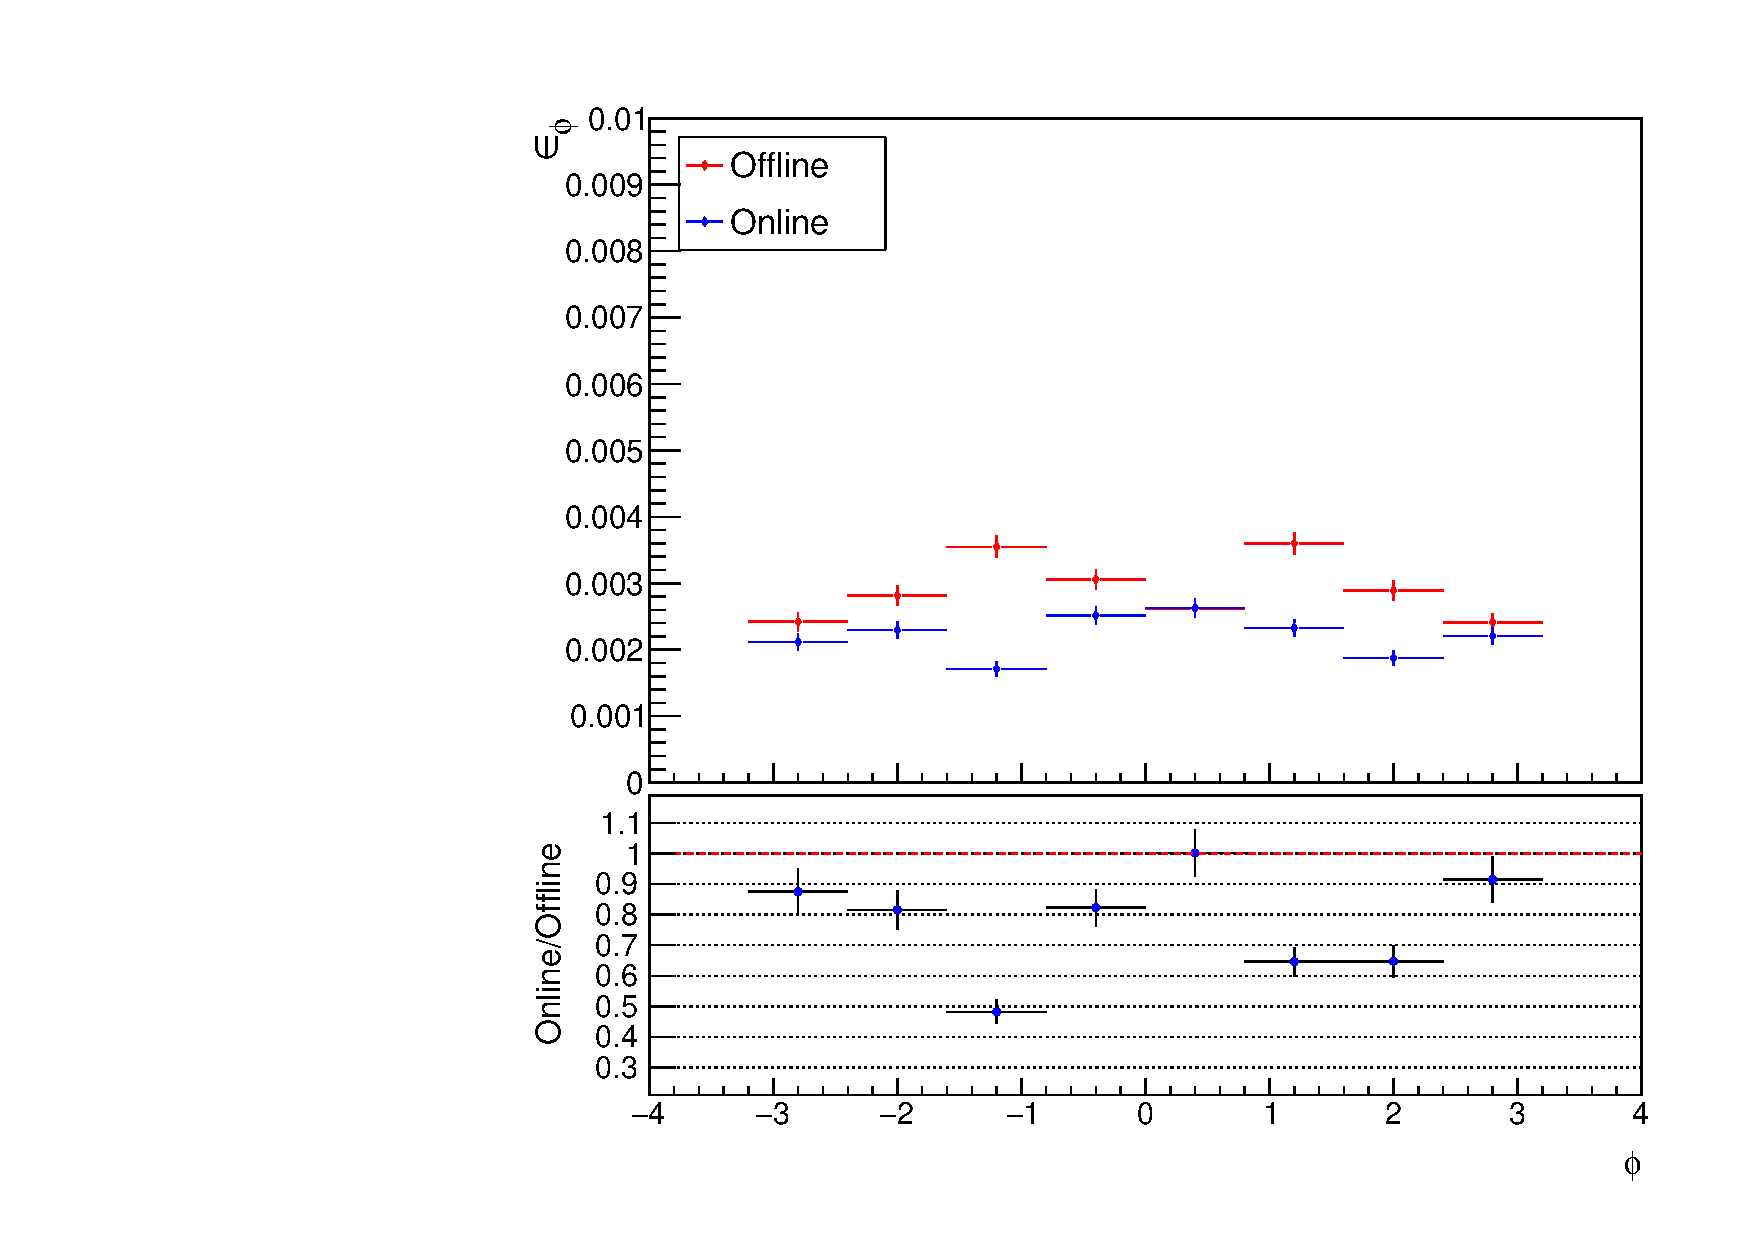
\includegraphics[width=1\linewidth]{phiLIGHTJET}
			\end{minipage}
			\caption{ }
			\label{fig:MC:lightjetefficiency}
		\end{figure}
	
	\subsection{Tag Matching}
	
	For each pair of jets that could be matched between online and offline, and then successfully have a $b$-tagging decision evaluated on the jets, the agreement of the $b$-tagging between the two jets was checked. These were found to match one another in $90.91\%$ of cases.
	
	\section{MV2 Discriminant Values - ???} \todo{Necessary}
	
	\note{Here would show plots of the MV2 value against pt/eta or whatever}
	
	\section{MV2 Input Variables - ???}


\endinput
